\documentclass[10pt,a4paper]{article}
\usepackage[utf8]{inputenc}
\usepackage[T1]{fontenc}
\usepackage[italian]{babel}
\usepackage[margin=2cm]{geometry}
\usepackage{graphicx}
\usepackage{float}
\usepackage{subcaption}
\usepackage{amsmath,amssymb}
\usepackage[font=small,skip=3pt]{caption}
\usepackage{xcolor}
\usepackage{listings}
\usepackage{hyperref}
\hypersetup{colorlinks=true,linkcolor=blue!50!black,citecolor=blue!50!black}

% --- cartella immagini: carica i PNG in una cartella "figures/" su Overleaf ---
\graphicspath{{figures/}{./}}

% --- stile codice Python per l'appendice ---
\definecolor{codegray}{gray}{0.95}
\definecolor{kw}{rgb}{0.0,0.2,0.6}
\definecolor{cmt}{rgb}{0.0,0.5,0.0}
\definecolor{str}{rgb}{0.6,0.0,0.0}
\lstset{
  language=Python, basicstyle=\ttfamily\scriptsize, backgroundcolor=\color{codegray},
  keywordstyle=\color{kw}\bfseries, commentstyle=\color{cmt}\itshape,
  stringstyle=\color{str}, numbers=left, numberstyle=\tiny\color{gray},
  breaklines=true, frame=single, framesep=3pt, showstringspaces=false, columns=fullflexible
}

\setlength{\parindent}{0pt}
\setlength{\parskip}{4pt}

\title{\vspace{-1.5em}\textbf{Self-Organised Criticality come modello di\\diffusione semantica sul lessico mentale}}
\author{Sebastiano Franchini}
\date{\vspace{-1em}\today}

\begin{document}
\maketitle
\vspace{-1.5em}

\textbf{Idea del progetto.} Molti sistemi neurali e cognitivi sembrano operare vicino a un punto critico:
le valanghe neuronali \cite{beggs2003} e l'ipotesi del ``cervello critico''
descrivono un'attività che si propaga in cascate \emph{senza scala caratteristica} (cioè senza una taglia "tipica": convivono eventi piccolissimi e valanghe enormi), un regime che rende il sistema molto reattivo. In questo lavoro ho provato a vedere se anche la diffusione semantica nel \emph{lessico mentale} si comporta in modo simile, proponendo un'alternativa ai classici modelli continui di \emph{spreading activation}.
Per farlo, ho mappato la rete di associazioni libere \textbf{SWOW-EN} \cite{dedeyne2019} su un \textbf{modello Sandpile Abeliano}: in questa simulazione, un "grano di sabbia" rappresenta un'unità di attivazione che si posa su una parola. Ogni parola (nodo) può accumulare grani fino a un certo limite, stabilito dal suo numero di connessioni (il suo \emph{grado}). Se supera questa soglia di tolleranza, il nodo diventa instabile e "crolla", cedendo un grano a ciascuno dei suoi vicini e innescando potenzialmente una reazione a catena (una \emph{valanga}).

\textbf{Come funziona} (Fig.~\ref{fig:anim}): per visualizzare la dinamica, in questo piccolo vicinato semantico ho iniettato i grani sempre sullo stesso nodo. L'attivazione si accumula finché il nodo supera la soglia e \emph{crolla}, passando i grani ai vicini e propagando la valanga.

\begin{figure}[htbp]
\centering
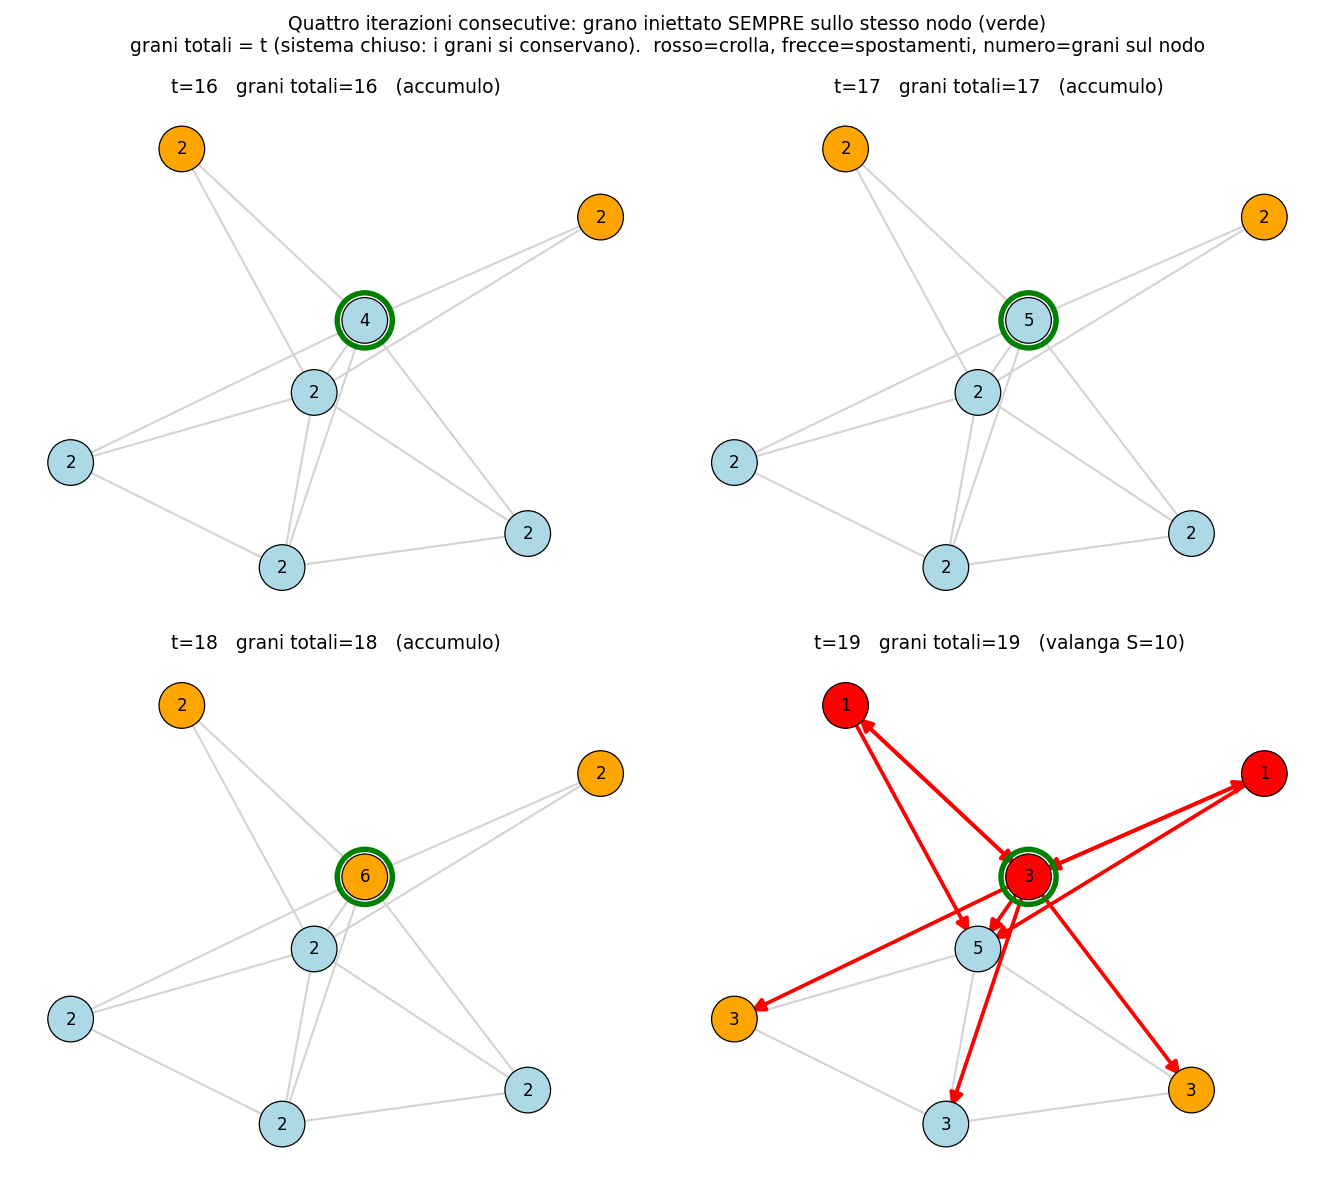
\includegraphics[width=0.85\textwidth]{soc_animation_frames.png}
\caption{Quattro iterazioni consecutive su un piccolo vicinato della rete SWOW. Il grano viene fatto cadere sempre sullo stesso nodo bersaglio. Si nota l'accumulo dei grani ($4\!\to\!5\!\to\!6$) fino al momento del crollo, che innesca la valanga e distribuisce l'attivazione ai vicini.}
\label{fig:anim}
\end{figure}

\section{Distribuzione delle valanghe a legge di potenza}
Per evitare che l'energia cresca all'infinito, ho usato un nodo ad alto grado come \emph{sink} (un pozzo che assorbe i grani in eccesso senza mai crollare). La grandezza chiave per studiare il sistema è la \emph{dimensione della valanga} $S$, cioè il numero totale di spostamenti di grani avvenuti in una singola cascata. 

Per capire quanto sono probabili le valanghe grandi, la Fig.~\ref{fig:soc}a mostra la distribuzione delle taglie in scala log-log. La disegno come densità di probabilità (PDF) con binning logaritmico, che è il modo standard di presentarla e non perde informazione nella coda. Il grafico è una retta in discesa di pendenza $-\alpha$: è il classico segnale di una legge di potenza, ma da solo non basta, perché anche altre distribuzioni possono dare un grafico simile. Con il test statistico di Clauset et al. (2009), tramite la libreria \texttt{powerlaw}, ho stimato un esponente $\alpha\!\approx\!1.44$ ($x_{\min}=14$, $95\%$ CI $[1.41, 1.47]$, $N=2917$ valanghe su un sottografo di $1500$ nodi). Il test del rapporto di verosimiglianza preferisce nettamente la legge di potenza rispetto all'esponenziale ($R=33.8, p\ll0.001$) e non riesce a distinguerla da una log-normale ($R=1.06, p=0.29$). Per onestà: una legge di potenza \emph{troncata} risulta anzi migliore di quella pura ($R=-4.16, p<0.001$), ma è normale --- in un sistema finito c'è sempre un taglio nella coda (la lieve risalita finale in Fig.~\ref{fig:soc}a). Insomma: le grandi reazioni a catena ci sono, ma la prova statistica di un regime \emph{scale-free} perfetto non è definitiva. Infine, ho provato a simulare cosa succede se ogni tanto qualche grano svanisce durante il crollo (probabilità di dissipazione $f>0$). Come si vede in Fig.~\ref{fig:soc}b, la curva cade improvvisamente verso il basso: le valanghe grandi smettono di avvenire.

\begin{figure}[htbp]
\centering
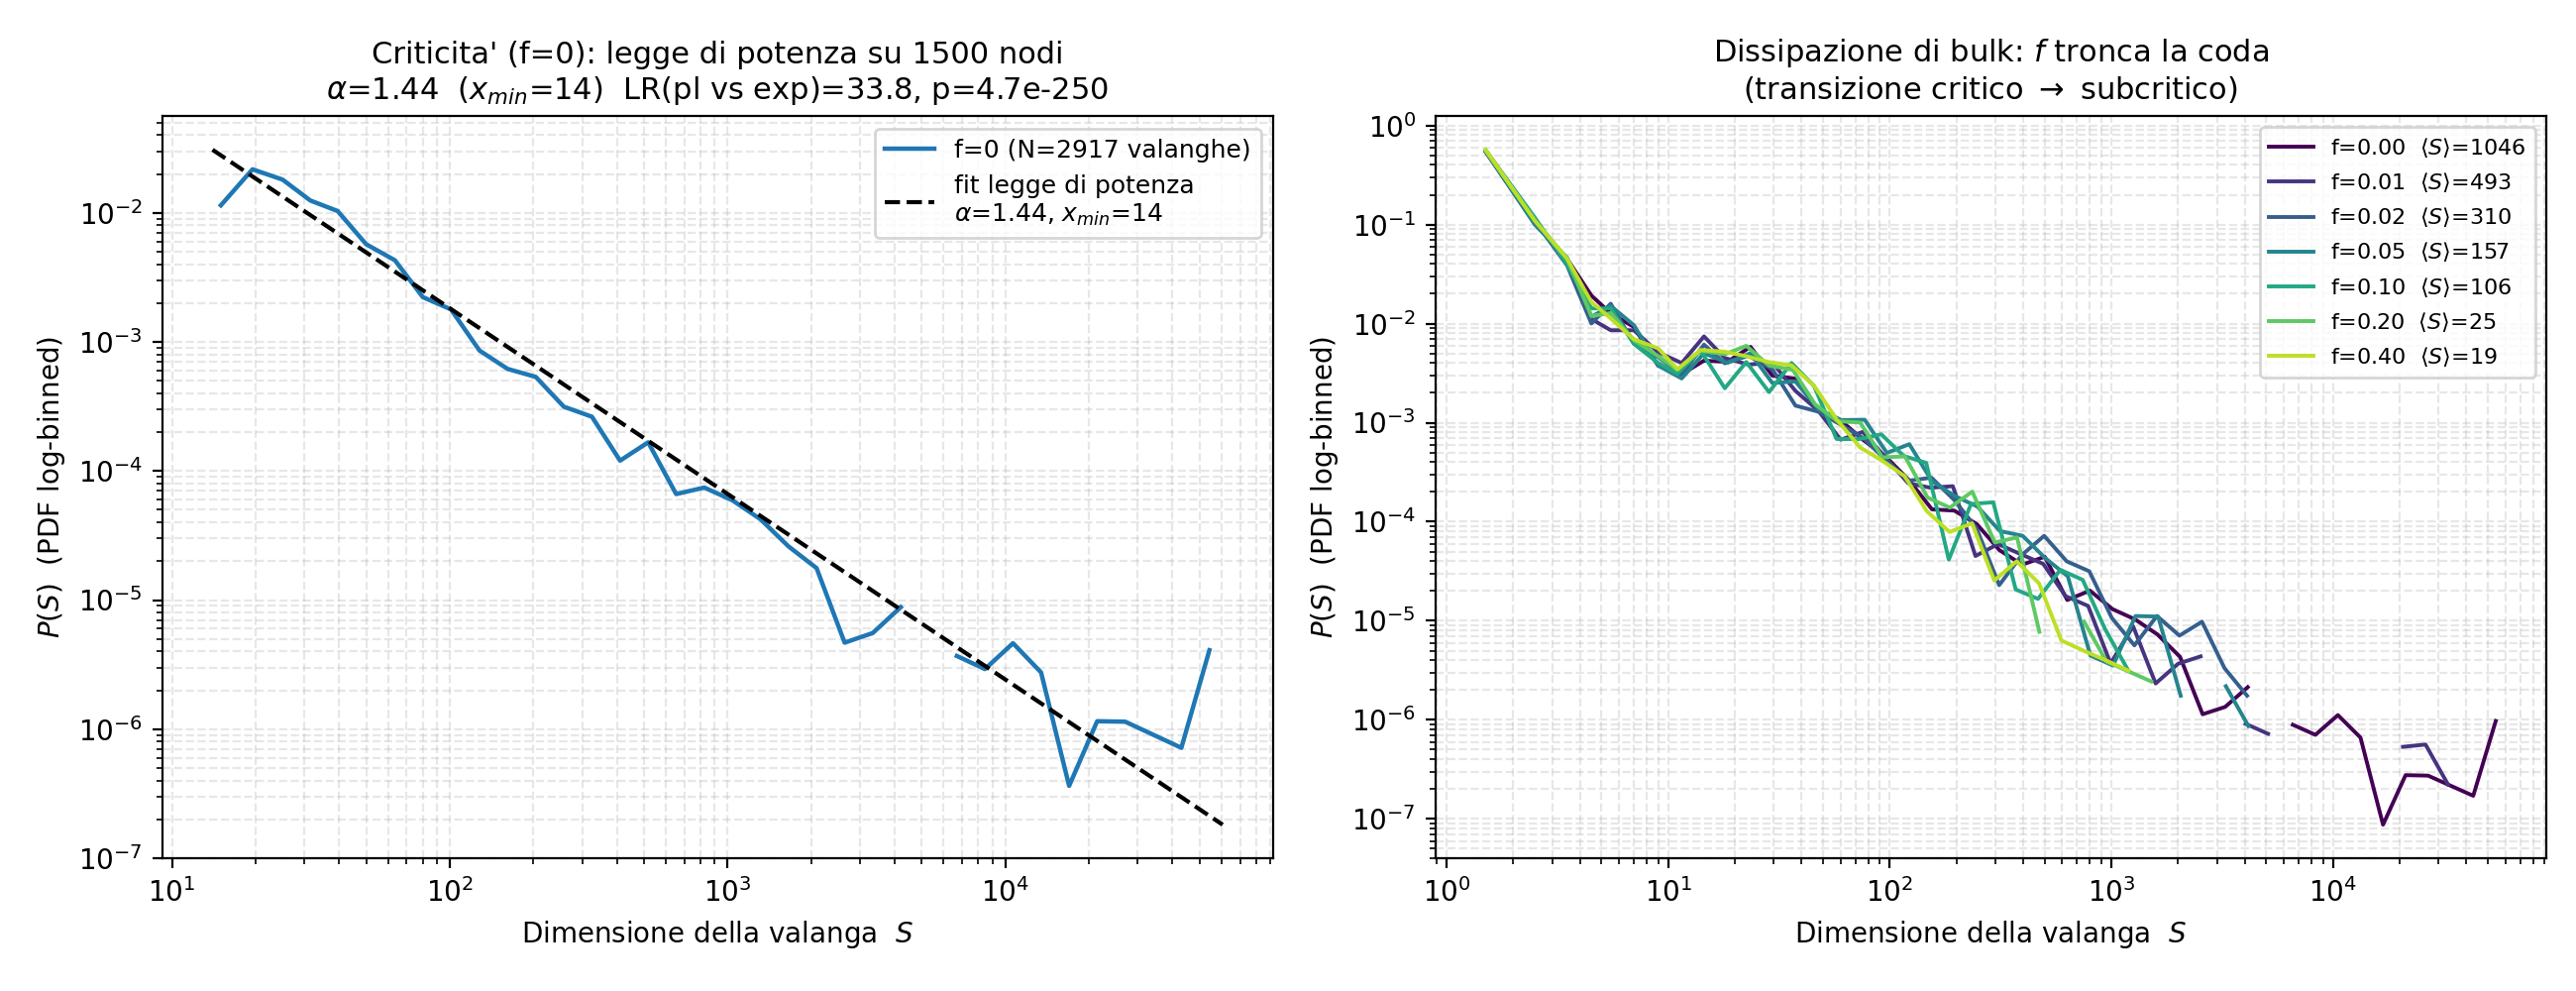
\includegraphics[width=0.85\textwidth]{soc_powerlaw_phase_transition.png}
\caption{Distribuzione delle dimensioni delle valanghe. In entrambi i pannelli, l'\textbf{asse X} rappresenta la dimensione della valanga $S$ (il numero totale di spostamenti di grani avvenuti prima che il sistema torni stabile) e l'\textbf{asse Y} la densità di probabilità $P(S)$ (PDF con binning logaritmico). \textbf{(a)} Senza dissipazione di bulk ($f=0$): si nota una retta in scala log-log di pendenza $-\alpha$, a indicare che non c'è una scala dominante (legge di potenza con $\alpha\!\approx\!1.44$); la lieve risalita finale è la deviazione di taglia finita. \textbf{(b)} Aumentando la probabilità di dissipazione $f$, la coda viene troncata sempre prima: il sistema passa a un regime subcritico dove le valanghe enormi sono soppresse.}
\label{fig:soc}
\end{figure}

\begin{figure}[htbp]
\centering
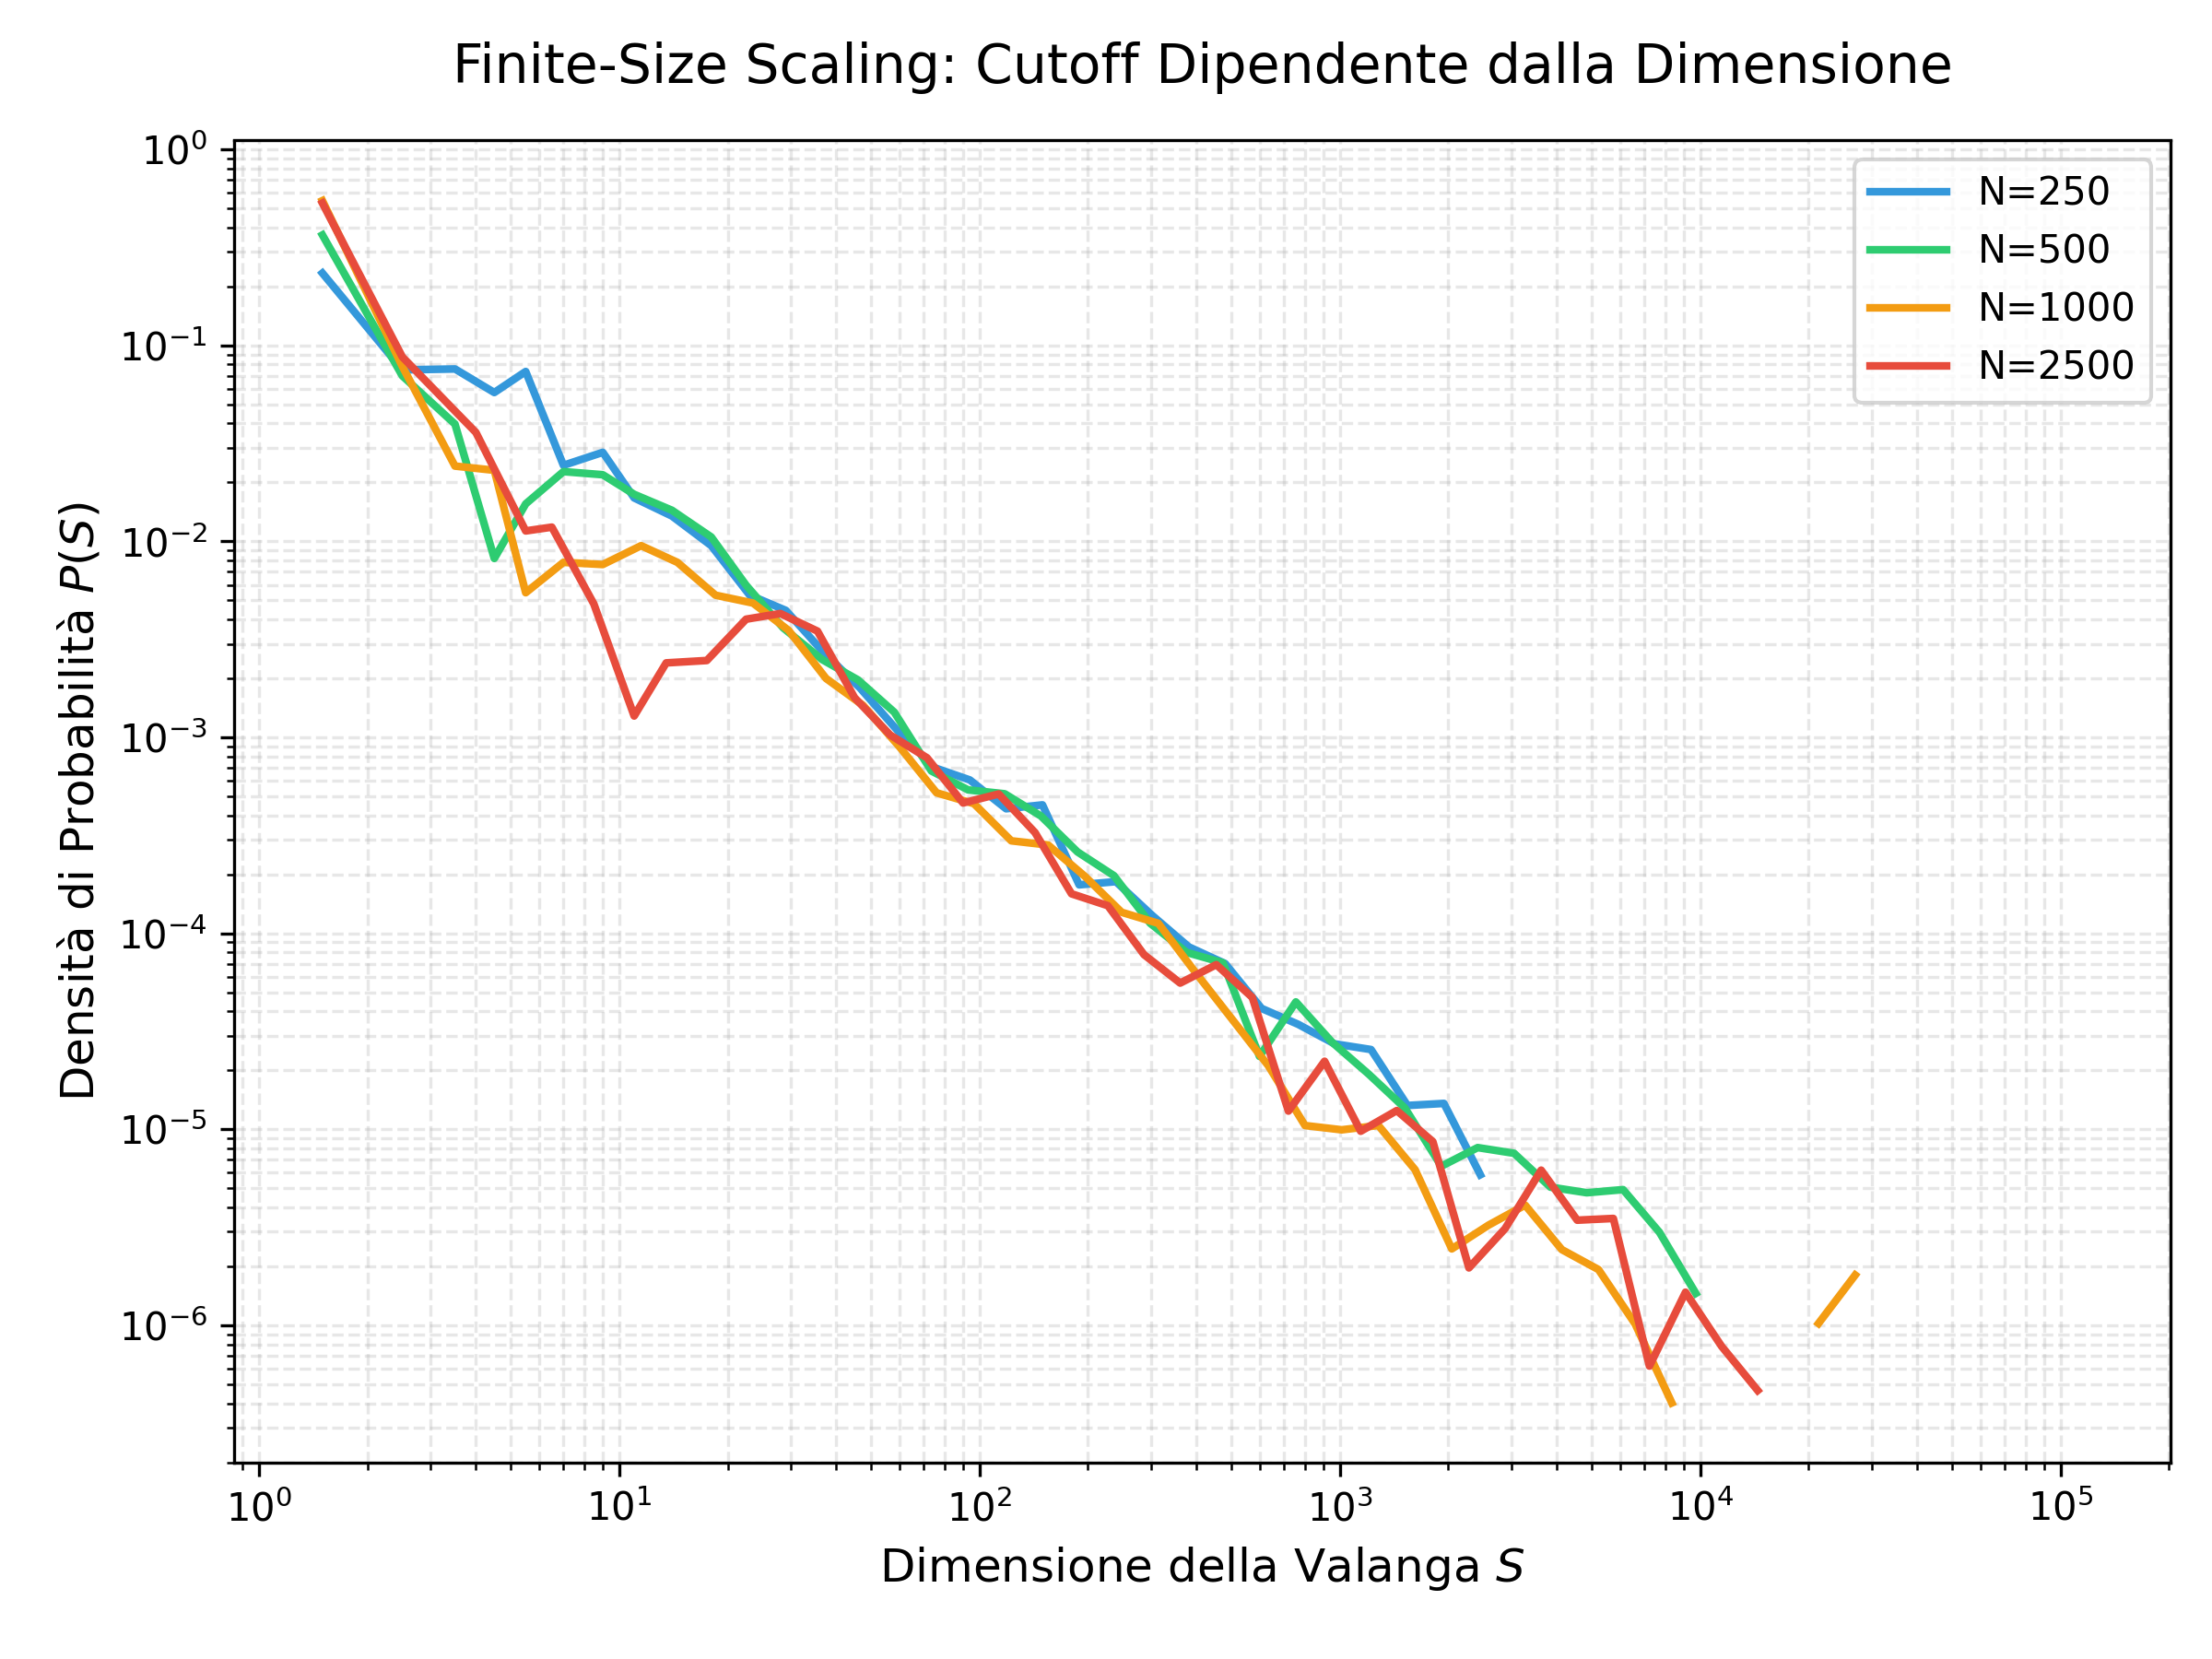
\includegraphics[width=0.85\textwidth]{finite_size_scaling.png}
\caption{Finite-size scaling. Distribuzione di probabilità (log-binned PDF) per sottoreti di dimensioni diverse ($N=250, 500, 1000, 2500$, campionate tramite esplorazione BFS dalla componente gigante). Le curve si sovrappongono lungo quasi tutto il dominio, segno di una regione a legge di potenza condivisa; tuttavia, su queste taglie e con sottografi annidati, il cutoff \emph{non} si sposta in modo chiaro al crescere di $N$ e non c'è un vero \emph{data collapse}. La FSS è quindi solo un indizio debole, non una prova: servirebbero sottografi indipendenti e una gamma di taglie più ampia.}
\label{fig:fss}
\end{figure}

\textbf{Perché è necessario il sink?} Senza un meccanismo di dissipazione il sistema è chiuso: i grani entrano e non escono mai, quindi la densità sale di continuo. Superata una certa densità il sistema non riesce più a stabilizzarsi e \emph{diverge} (Fig.~\ref{fig:why}), con valanghe che non si fermano. Non è un guasto, però: è la stessa transizione di fase della sezione dopo. La divergenza è l'ingresso nella \emph{fase attiva}, il regime in cui l'attività si autoalimenta --- il caos comincia proprio dove l'analisi con il sink si ferma. Il sistema, tra l'altro, diverge \emph{prima} di riempirsi del tutto (prima della somma dei gradi, che è il massimo teorico). Il sink scarica i grani in eccesso e riporta tutto a uno stato stazionario, dove ha senso calcolare le statistiche.

\begin{figure}[htbp]
\centering
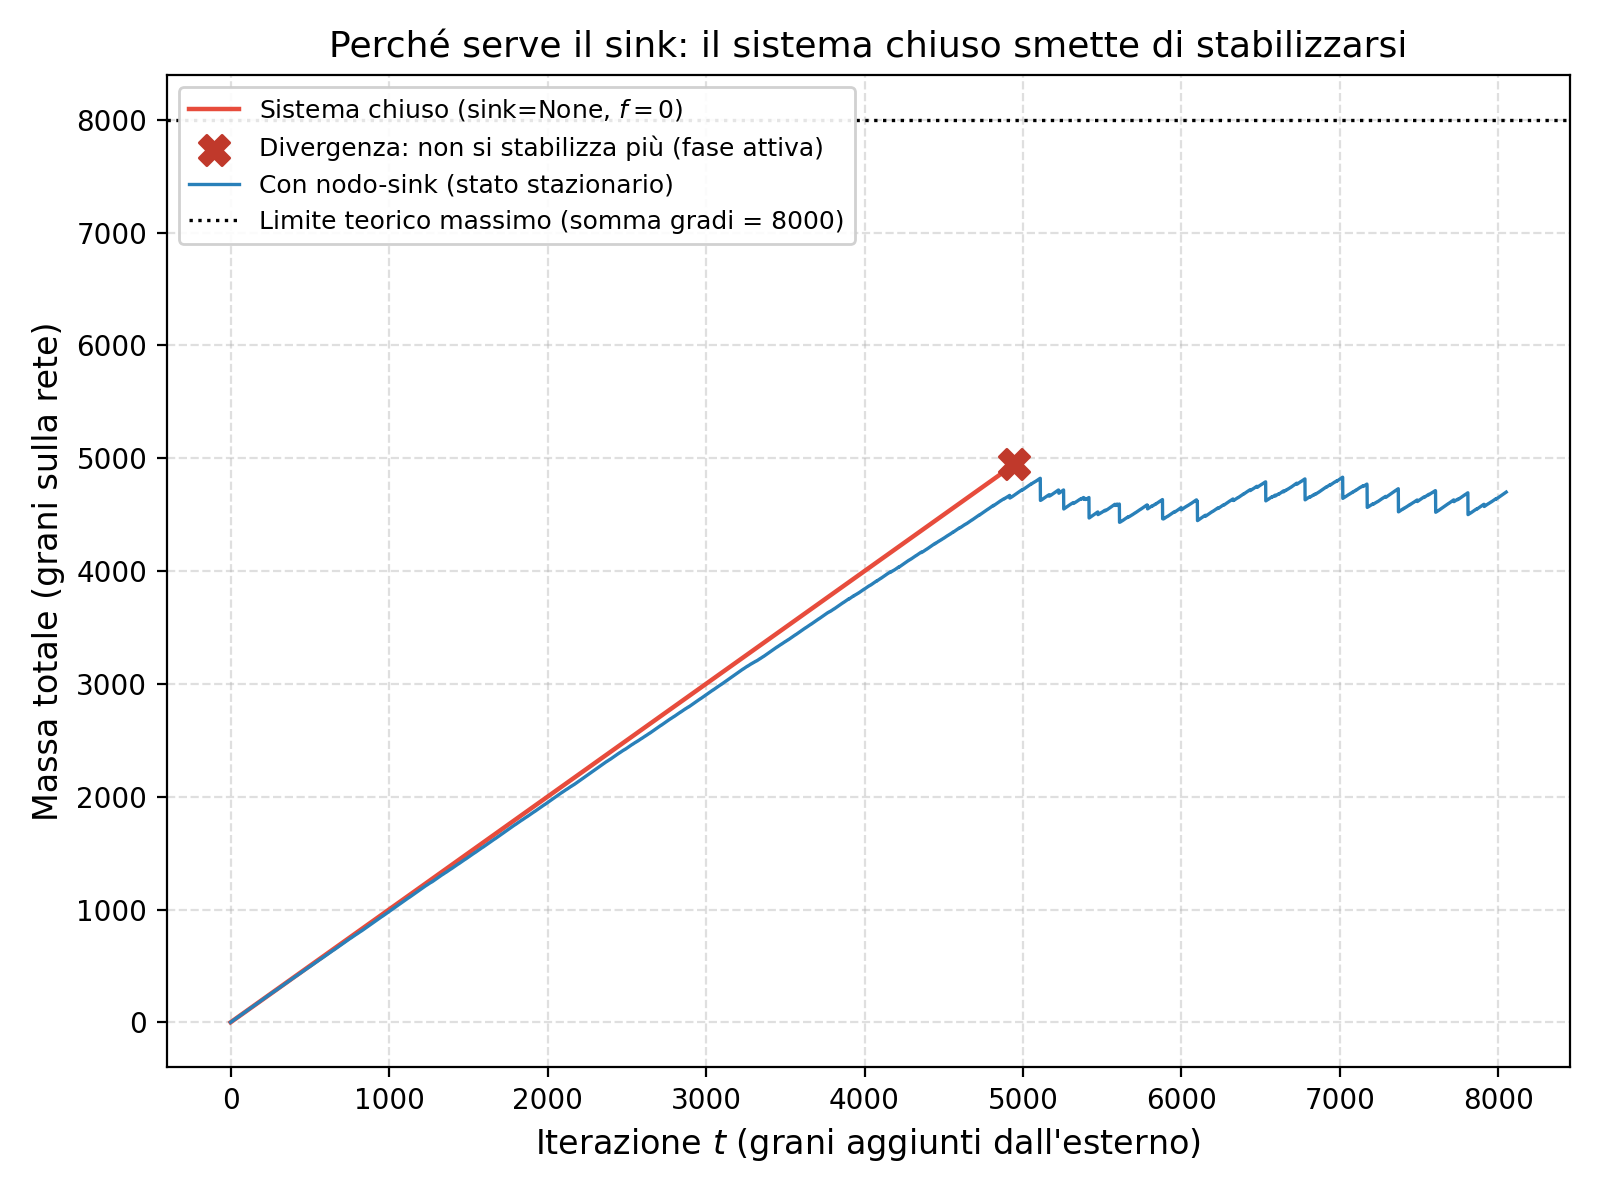
\includegraphics[width=0.85\textwidth]{soc_why_sink.png}
\caption{Evoluzione della massa totale nel tempo. Sull'\textbf{asse X} c'è il tempo (misurato in iterazioni, ossia in numero di grani iniettati dall'esterno) e sull'\textbf{asse Y} la massa (il numero totale di grani fisicamente presenti sull'intera rete). Dal grafico si evince che senza sink i grani si accumulano all'infinito e la curva della massa diverge. Aggiungendo un nodo-sink, invece, la massa si appiattisce su un valore stazionario, condizione necessaria per lo studio delle valanghe.}
\label{fig:why}
\end{figure}

\section{Transizione di fase e auto-organizzazione}
In fisica statistica la SOC si può vedere come una vera transizione di fase. Per studiarla guardo due grandezze: il parametro che "spinge" il sistema, cioè la \textbf{densità di grani} $\rho$ (grani totali diviso numero di nodi), e quello che ne risulta, cioè l'\textbf{attività} stazionaria $\rho_a$ (la frazione di nodi che sta crollando in un dato istante).
Come si vede in Fig.~\ref{fig:trans}a, sotto una certa densità critica $\rho_c$ i crolli si fermano in fretta e l'attività si spegne (fase assorbente), mentre superata la soglia il sistema "si accende" e l'attività continua nel tempo (fase attiva). Dai dati la transizione sembra avvenire attorno a $\rho_c\!\approx\!2.1$ (poco più di 2 grani per nodo). Il fatto che questo numero ricordi la soglia del classico reticolo 2D ($\rho_c \approx 2.125$) è quasi certamente solo una coincidenza, legata a come ho definito la densità media su una rete così irregolare, e non un segno di fisica condivisa: su sottografi diversi otterrei soglie diverse. Il pannello (b) mostra proprio l'andamento nel tempo dell'attività.

Un aspetto interessante del modello (Fig.~\ref{fig:iter}) è che, partendo da una rete vuota e aggiungendo i grani lentamente (uno alla volta), la densità di grani $\rho(t)$ sale da zero e si assesta spontaneamente su un valore stazionario, senza dover fissare a mano la densità iniziale. È il \emph{meccanismo} dell'auto-organizzazione (drive lento $+$ dissipazione $\to$ stato stazionario). C'è però un limite importante, che dico apertamente: il valore stazionario raggiunto \emph{non} coincide con la densità critica $\rho_c$ della transizione di fase. Quindi la predizione forte della teoria SOC \cite{dickman2000}, cioè "densità auto-organizzata $=\rho_c$", su questa rete non è rispettata (vedi didascalia).

\begin{figure}[htbp]
\centering
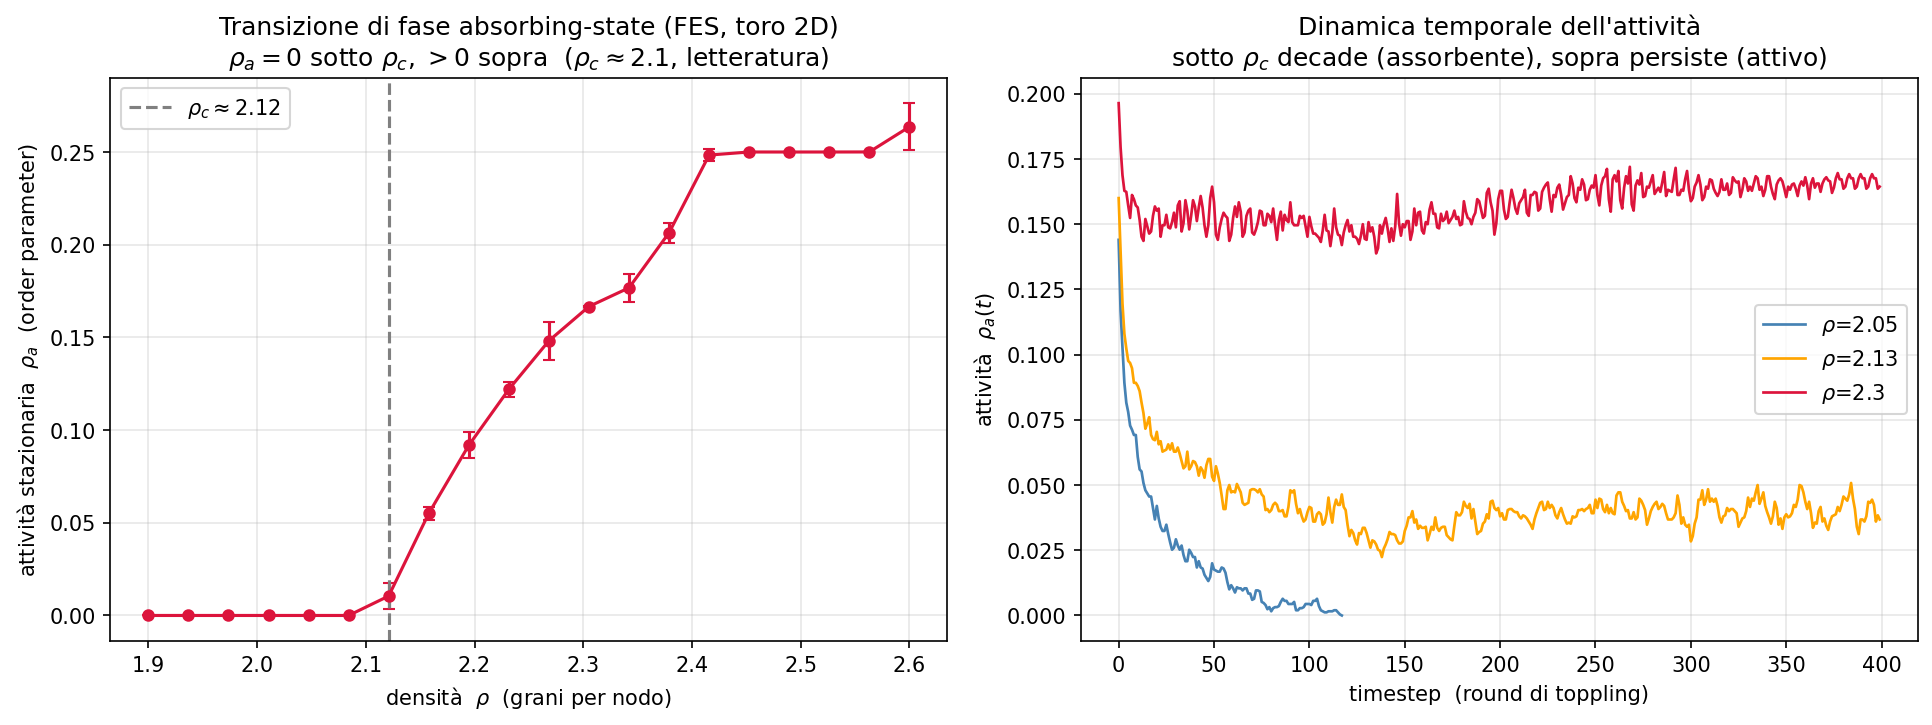
\includegraphics[width=0.85\textwidth]{soc_phase_transition.png}
\caption{Transizione di fase (simulazione su un sottografo di $N=1000$ nodi estratto via BFS). \textbf{(a)} Sull'\textbf{asse X} c'è la densità di grani $\rho$ (quanti grani ci sono in media per ogni nodo) e sull'\textbf{asse Y} l'attività stazionaria $\rho_a$ (la frazione percentuale di nodi in stato di crollo). Il grafico mostra chiaramente che sotto la densità critica $\rho_c\!\approx\!2.1$ l'attività muore, mentre superata la soglia il sistema "si accende" mantenendo valanghe perpetue. \textbf{(b)} Dinamica nel tempo: l'\textbf{asse X} è il tempo e l'\textbf{asse Y} è l'attività $\rho_a$. Nelle simulazioni sotto soglia l'attività decade rapidamente a zero, mentre in quelle sopra soglia l'attività persiste indefinitamente.}
\label{fig:trans}
\end{figure}

\begin{figure}[htbp]
\centering
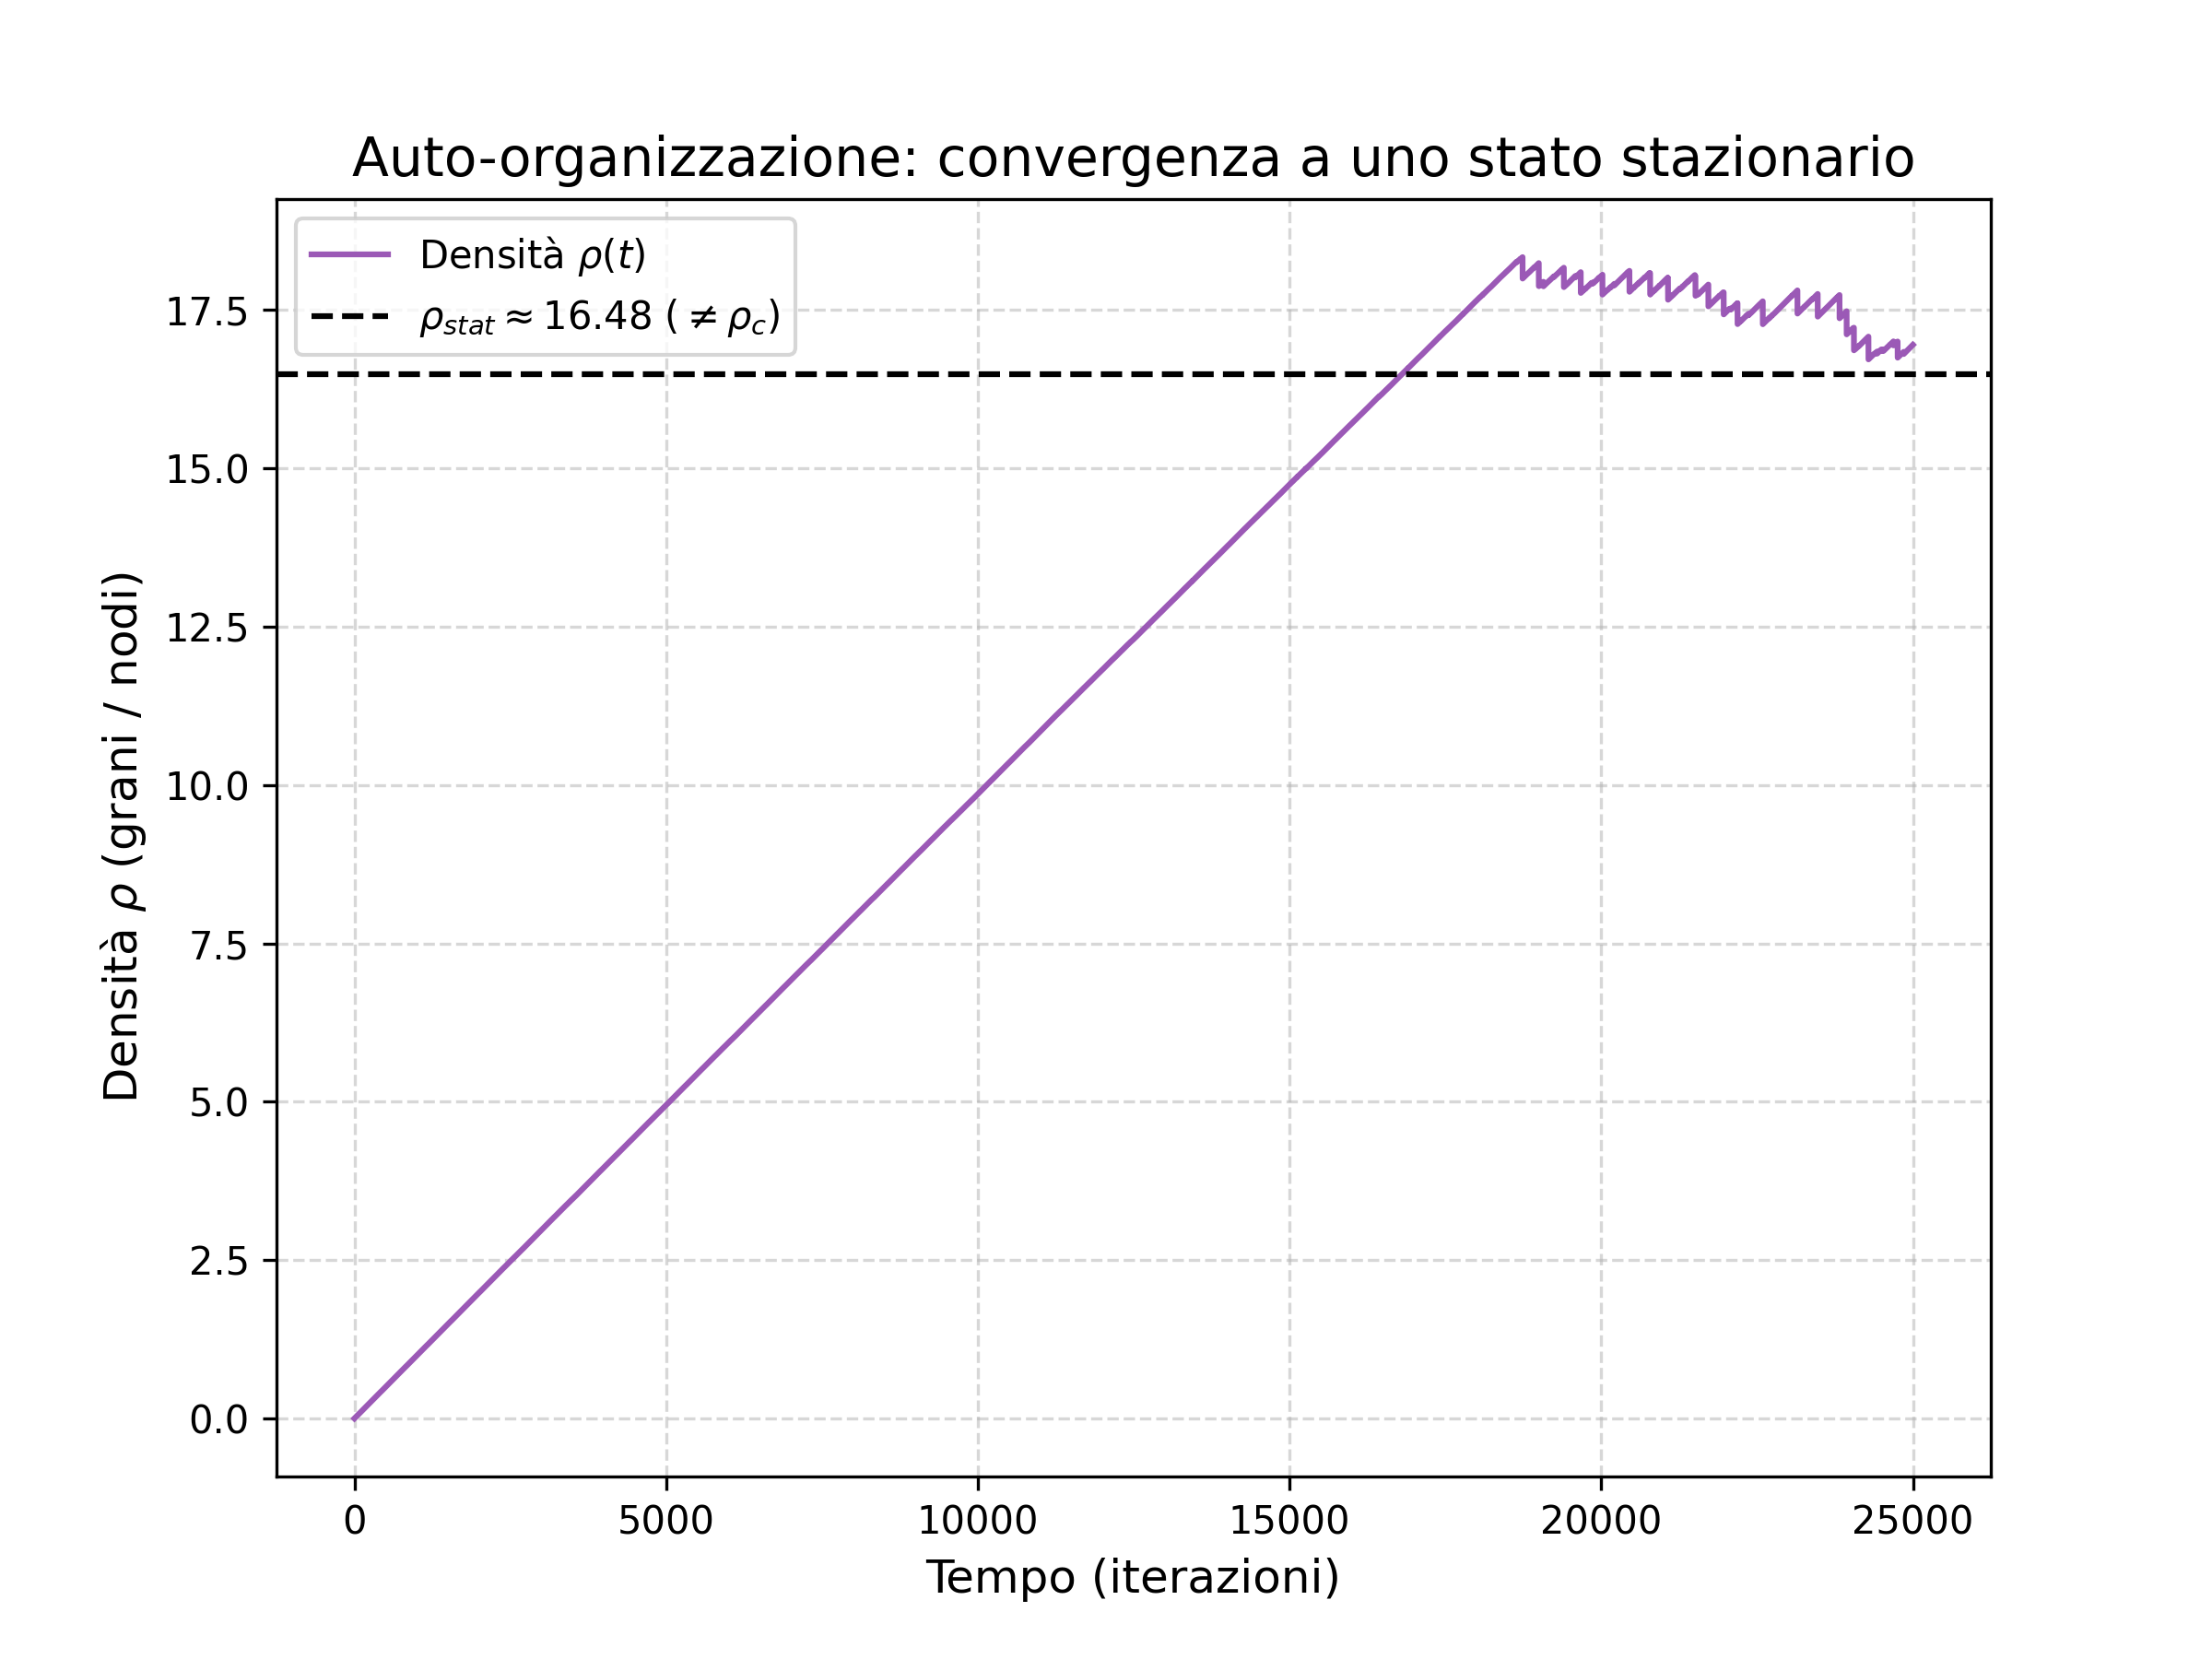
\includegraphics[width=0.85\textwidth]{soc_rho_vs_time.png}
\caption{Auto-organizzazione su un sottografo SWOW ($N=1000$, lo stesso della transizione di fase). L'\textbf{asse X} indica il tempo (iterazioni), l'\textbf{asse Y} la densità di grani $\rho(t)$. Partendo da zero, la densità converge spontaneamente verso un asintoto stazionario, illustrando il meccanismo dell'auto-organizzazione. L'asintoto si attesta però a $\rho\approx 16.4$, cioè circa \emph{metà del grado medio} della rete ($\langle k\rangle\!\approx\!31$), e \emph{non} coincide con la densità critica $\rho_c\!\approx\!2.1$ stimata dalla transizione di fase. Il valore stazionario dipende quindi dalla topologia (grado medio del sottografo) e non rappresenta una densità critica universale: l'identificazione SOC ``densità stazionaria $=\rho_c$'' qui non regge.}
\label{fig:iter}
\end{figure}

\section{Una conseguenza cognitiva: il fan effect}
Cercando un riscontro sul piano cognitivo (Fig.~\ref{fig:fan}) ho verificato se i nodi-hub (molto interconnessi) inneschino valanghe più grandi quando vengono attivati. Usando un \emph{probe non distruttivo} (aggiungo un singolo grano al nodo bersaglio a partire dallo stato stazionario e ripristino il background dopo ogni prova, così da non contaminare le misure tra nodi diversi), il risultato è \textbf{negativo}: la correlazione di Spearman tra grado e taglia media della valanga è $\rho_s\!\approx\!-0.30$ ($p\!\approx\!10^{-11}$) e la correlazione parziale con la betweenness, controllando per il grado, è praticamente nulla ($\rho_{\text{partial}}\!\approx\!-0.03$).
Ha senso dal punto di vista fisico: nel modello la soglia di un nodo \emph{è} il suo grado, quindi gli hub sono proprio i nodi più \emph{difficili} da far crollare con una sola attivazione (sono robusti), mentre i nodi periferici a basso grado superano subito la soglia.
In altre parole, l'analogia con l'\textbf{effetto fan} \cite{anderson1974} --- l'idea che un concetto con molte associazioni disperda di più l'attivazione --- da questo sandpile \emph{non} viene fuori da sola. Un effetto fan apparente si ottiene solo stimolando lo stesso nodo molte volte di fila, ma è un artefatto dell'accumulo forzato, non una vera proprietà cognitiva del modello.

\begin{figure}[htbp]
\centering
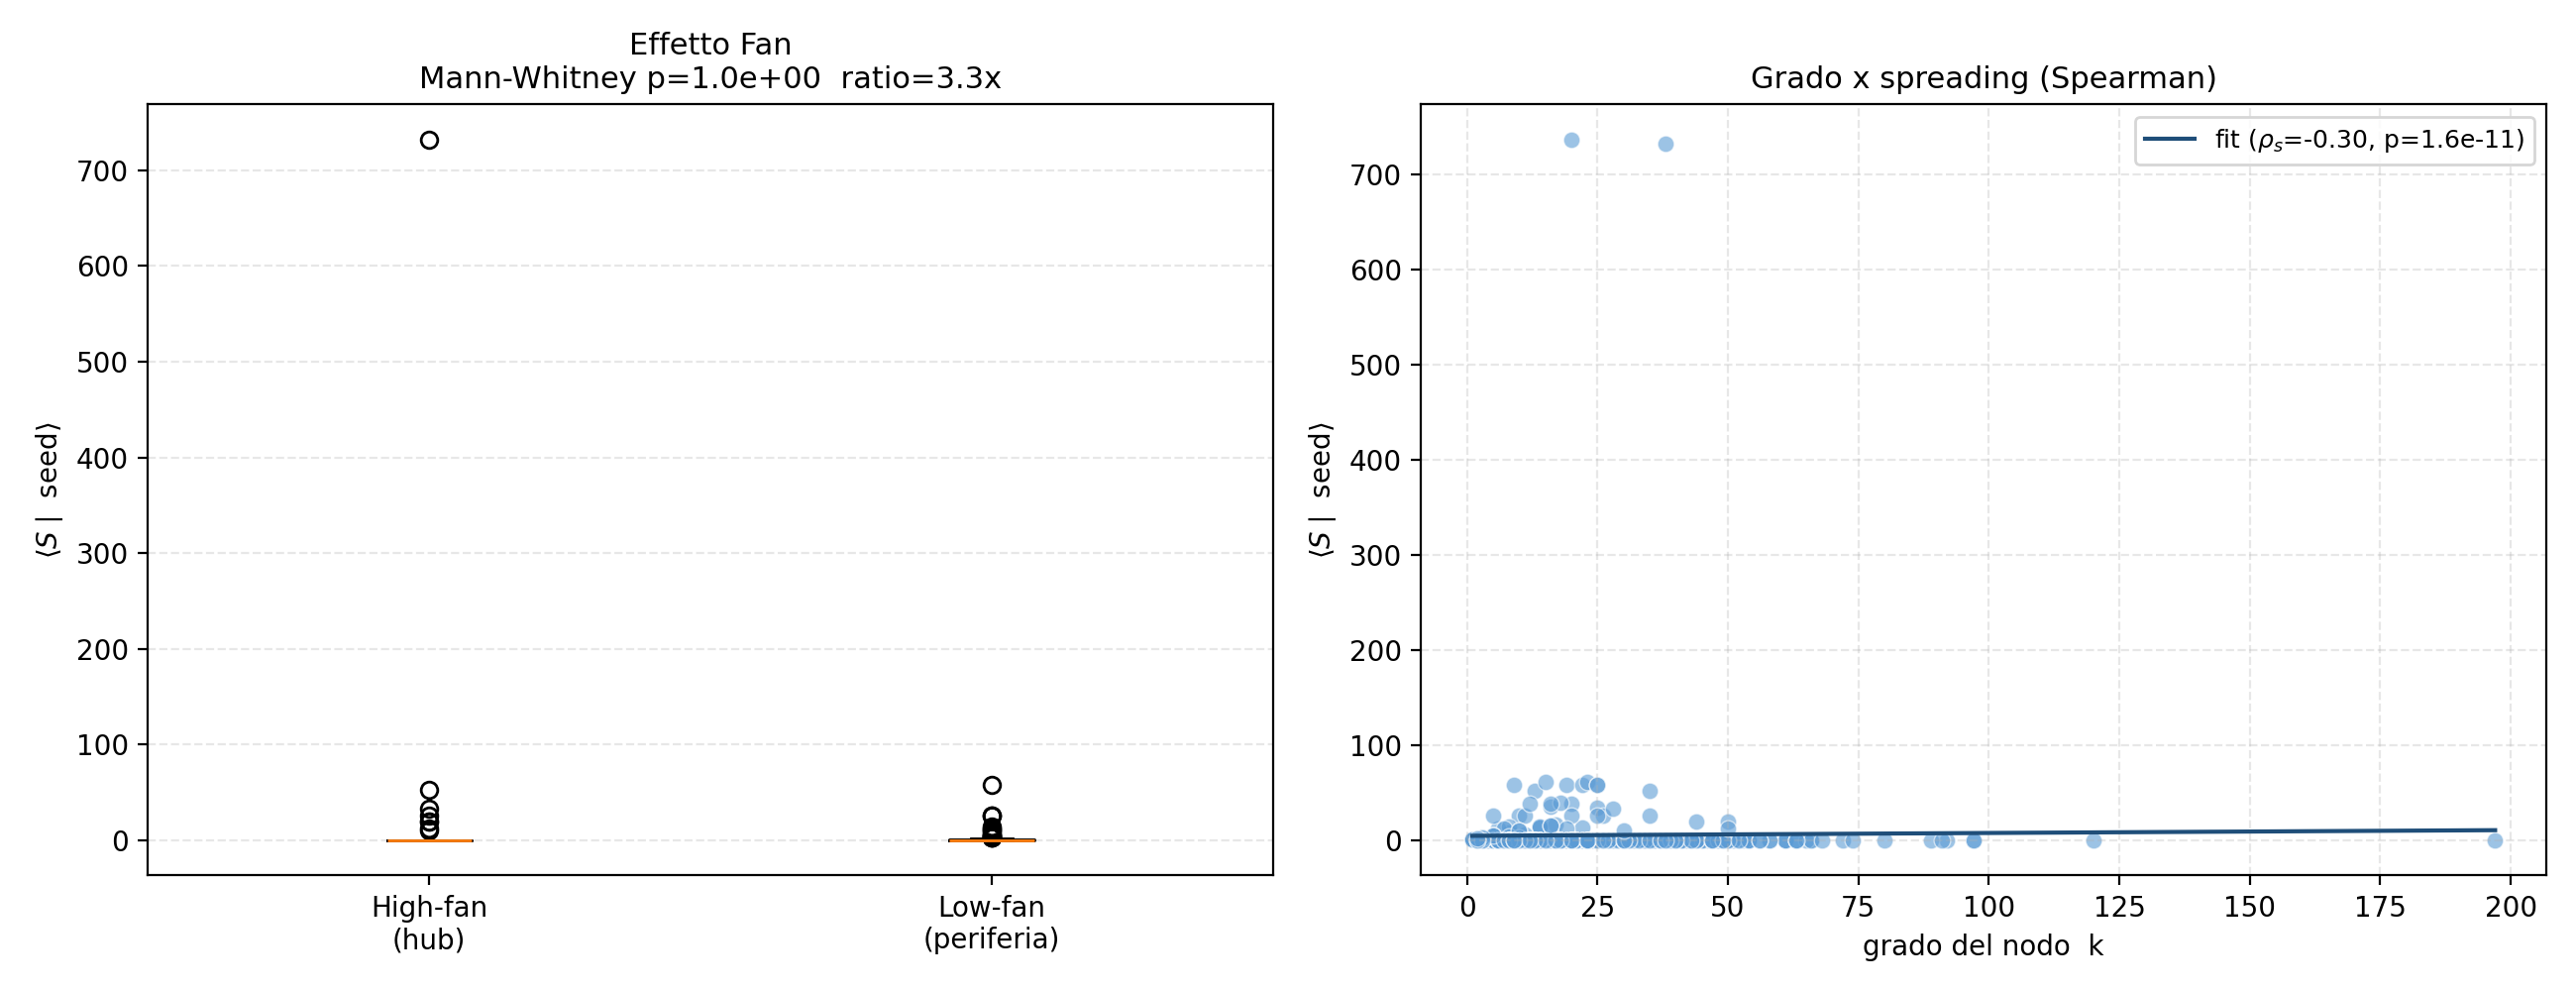
\includegraphics[width=0.85\textwidth]{fan_effect_sandpile.png}
\caption{Effetto fan (probe non distruttivo, sottografo $N=500$). \textbf{A sinistra}: distribuzione della taglia media di valanga $\langle S\mid$seed$\rangle$ per nodi hub vs periferici; le due categorie sono di fatto indistinguibili (Mann--Whitney non significativo). \textbf{A destra}: grado del nodo (\textbf{asse X}) contro taglia media della valanga (\textbf{asse Y}). Non c'è alcuna crescita con il grado: la correlazione di Spearman è anzi leggermente negativa ($\rho_s\!\approx\!-0.30$). Le valanghe più grandi sono innescate da nodi a grado medio-basso, non dagli hub, che essendo ad alta soglia risultano robusti alla singola attivazione.}
\label{fig:fan}
\end{figure}

\section{Un'applicazione predittiva: il Priming Semantico}
A cosa serve, in pratica, questo modello? Per provarlo, ho testato il Sandpile sui dati reali del Semantic Priming Project. La domanda era: il tempo che il Sandpile impiega a far crollare una parola bersaglio è legato al tempo di reazione misurato nelle persone? Su un campione piccolo ($N=169$, Fig.~\ref{fig:priming}), il tempo del Sandpile si correla con i tempi umani in modo debole e non significativo ($\rho \approx -0.15, p = 0.0538$): spiega solo il 2.2\% della varianza, quindi l'effetto pratico è minimo. Batte sì la semplice distanza minima sul grafo (shortest path, $\rho \approx -0.03, p \approx 0.72$), ma va detto che contare i salti sul grafo è un avversario facile da superare, rispetto a distanze pesate o ai vettori semantici moderni.

\begin{figure}[htbp]
\centering
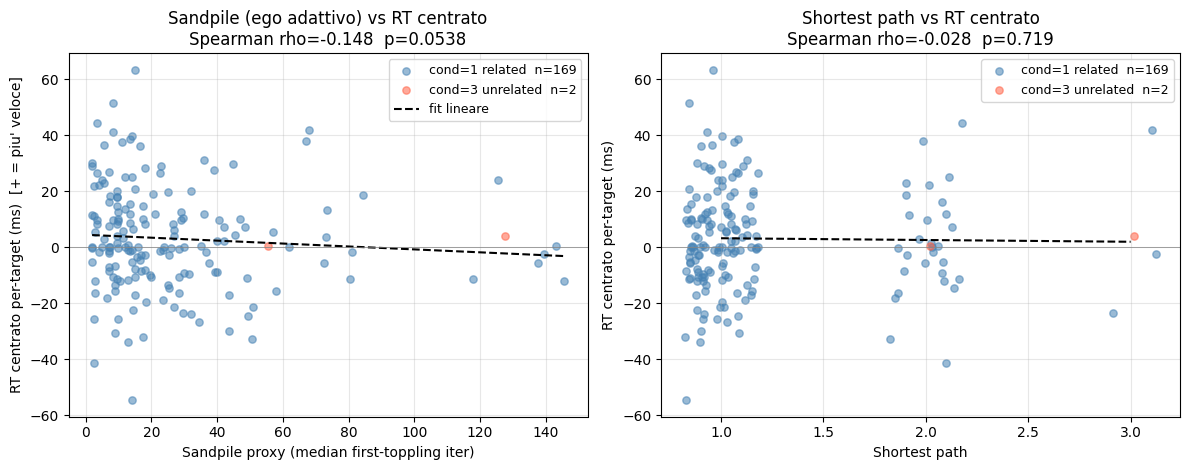
\includegraphics[width=0.85\textwidth]{spp_priming_validation.png}
\caption{Validazione empirica. In entrambi i pannelli, l'\textbf{asse Y} rappresenta l'effetto di priming in millisecondi (la facilitazione cognitiva: quanto l'umano è stato più veloce a rispondere rispetto alla sua media). \textbf{A sinistra}: l'\textbf{asse X} è il numero di step matematici (iterazioni) del Sandpile necessari all'attivazione per far crollare la parola bersaglio. La correlazione negativa misurata ($\rho \approx -0.15$) e il suo $p$-value ($p=0.0538$) indicano che se il Sandpile è "veloce" a trovare la parola, anche il cervello umano tende a esserlo. \textbf{A destra}: usando come predittore la classica distanza Shortest Path (il numero minimo di "salti" sul grafo, \textbf{asse X}), i punti sono del tutto dispersi e la correlazione scende a zero ($\rho \approx -0.03, p=0.72$): il Sandpile cattura quindi una dinamica non visibile dalla pura topologia statica.}
\label{fig:priming}
\end{figure}

\section{Limiti e semplificazioni del modello}
Prima di espandere questo approccio, è importante discutere alcuni limiti strutturali e le semplificazioni che ho dovuto introdurre:
\begin{itemize}
    \item \textbf{Topologia Non Orientata}: Per poter usare il modello Sandpile su questo grafo $G=(V,E)$, ho dovuto assumere che i legami fossero bidirezionali. Questa scelta sacrifica la reale asimmetria del lessico mentale (se la parola A fa venire in mente B, non è detto che valga il contrario con la stessa forza). Tuttavia, è un compromesso ragionevole: il sandpile classico (BTW) e i suoi strumenti di analisi sono pensati per grafi non orientati. La proprietà \emph{abeliana} (il risultato di una valanga non dipende dall'ordine dei crolli) vale anche sui grafi orientati \cite{dhar1990}, ma la versione simmetrica è la più semplice da studiare. L'asimmetria reale è recuperata separatamente con il modello stocastico di Manna (sezione finale).
    \item \textbf{La questione ``No Sink e $f=0$''}: Come mostrato nella \textbf{Figura \ref{fig:why}}, un sistema completamente chiuso (senza sink e senza dissipazione, $f=0$) su una rete finita non può fisicamente raggiungere uno stato stazionario: superata una certa massa la configurazione non ammette più una stabilizzazione finita. L'inserimento di un nodo sink non è quindi un trucco arbitrario, ma un requisito imposto dalla fisica statistica per permettere al sistema di assestarsi e poter studiare le valanghe.
    \item \textbf{Saturazione Globale e Divergenza}: Rimuovendo il sink, la rete si riempie fino a raggiungere un punto in cui la configurazione non ammette più una stabilizzazione finita. Nel codice, questa instabilità viene intercettata dal parametro \texttt{max\_topplings} per evitare blocchi computazionali. Tuttavia, non si tratta di un'euristica arbitraria: in un sistema chiuso la massa stabile non può superare la somma dei gradi $\sum_{v} \deg(v)$ (oltre quel valore non esiste nessuna configurazione stabile). In pratica però il sistema diverge anche \emph{prima}: appena la densità entra nella fase attiva, le valanghe non si fermano più. Non è un falso allarme del guard: l'ho verificato alzando \texttt{max\_topplings} fino a $2\times10^6$. Il nodo-sink serve proprio a scaricare questa sovra-eccitazione. Guardando quanto tempo ci mette a bloccarsi (Fig.~\ref{fig:divergence}), emerge che stimolare un hub porta la rete al limite termodinamico più in fretta ($\rho_s = -0.43$).
    \item \textbf{Forza del Segnale Comportamentale}: La correlazione predittiva calcolata sui dati umani ($\rho \approx -0.15$) indica un trend marginale ($p=0.0538$). Non volevo creare il predittore perfetto, ma fare un semplice \emph{proof-of-concept}: contare i crolli estrae un po' di segnale psicologico che distanze topologiche elementari come lo shortest path si perdono completamente.
    \item \textbf{Sviluppi Futuri (Asimmetria)}: Per superare il limite dei legami bidirezionali, la naturale estensione consiste nell'usare il Modello di Manna. Invece di crolli fissi e simmetrici, l'energia viene distribuita in modo stocastico, rispettando i pesi e la reale direzionalità delle associazioni.
\end{itemize}

\begin{figure}[htbp]
\centering
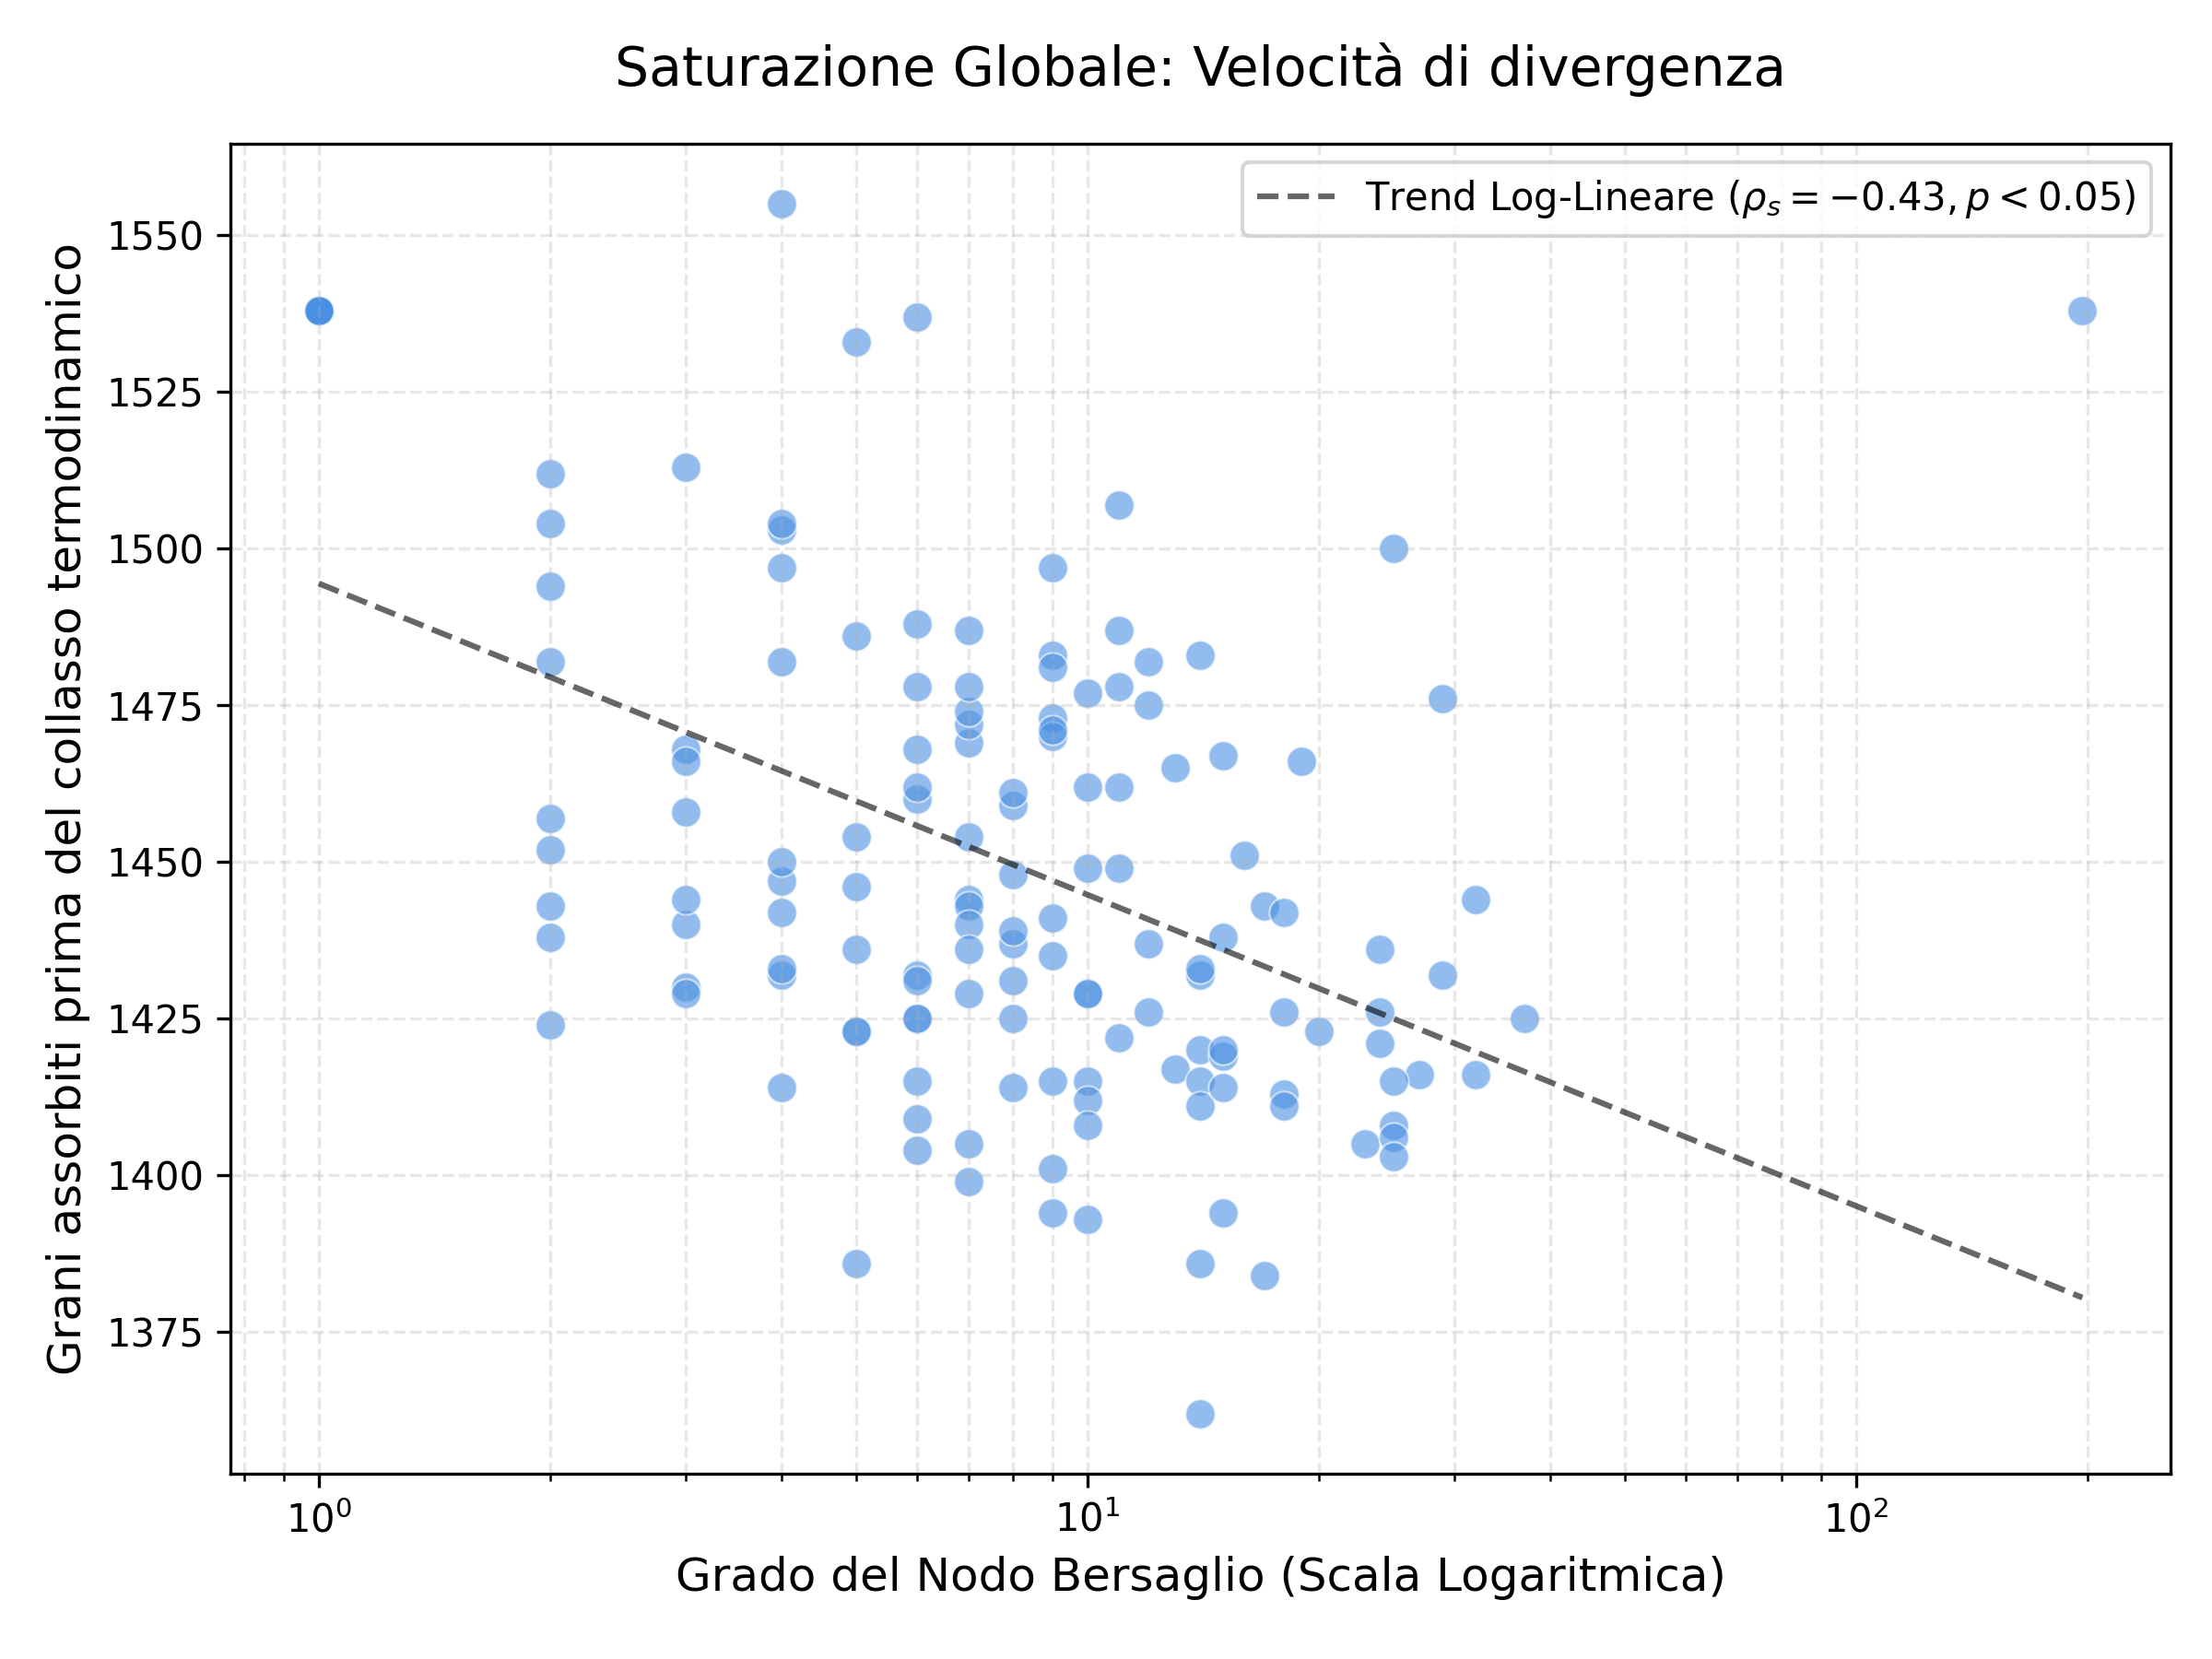
\includegraphics[width=0.85\textwidth]{soc_divergence_capacity.png}
\caption{Capacità di assorbimento della rete prima della divergenza. Iniettare attivazione esclusivamente in un nodo altamente connesso (hub) porta la rete al collasso termodinamico più rapidamente rispetto alla stimolazione di un nodo periferico ($\rho_s = -0.43$), suggerendo il ruolo degli hub come \emph{broadcaster} macroscopici.}
\label{fig:divergence}
\end{figure}

\textbf{In conclusione.} I risultati mostrano che la diffusione semantica ha alcuni tratti che ricordano la Self-Organised Criticality: caricare e scaricare energia a scatti somiglia a quello che fanno i sistemi neurali, e le taglie delle valanghe seguono curve compatibili con una legge di potenza (anche se è difficile distinguerla da una log-normale o da una legge di potenza troncata). Restano però dei limiti, che preferisco dire chiaramente: la densità a cui il sistema si auto-organizza dipende dalla rete e non coincide con la densità critica, e l'effetto fan sparisce quando lo si misura nel modo corretto. Il modello quindi è un \emph{proof-of-concept} interessante, non una prova definitiva che il lessico mentale sia critico.

\section{Verso l'asimmetria biologica: Il Sandpile Stocastico}
Per verificare che forzare la simmetria non abbia falsato tutto, ho fatto un test rapido (Fig.~\ref{fig:manna}) provando il \textbf{Modello di Manna} (1991) sulla vera rete SWOW asimmetrica. Qui, quando un nodo crolla, distribuisce i grani in modo stocastico proporzionalmente al peso reale dell'associazione umana. Anche con questa variante, le valanghe seguono stabilmente una legge di potenza. L'esponente però sale a $\alpha \approx 2.06$, molto diverso dall'$\alpha \approx 1.44$ della versione precedente. Aggiungere asimmetria e pesi sposta dunque in modo netto l'esponente; un singolo sottografo non basta per dichiarare formalmente una diversa \emph{classe di universalità}, ma lo spostamento è marcato e coerente con il fatto che i modelli di Manna e BTW sono ritenuti distinti in letteratura.

\begin{figure}[htbp]
\centering
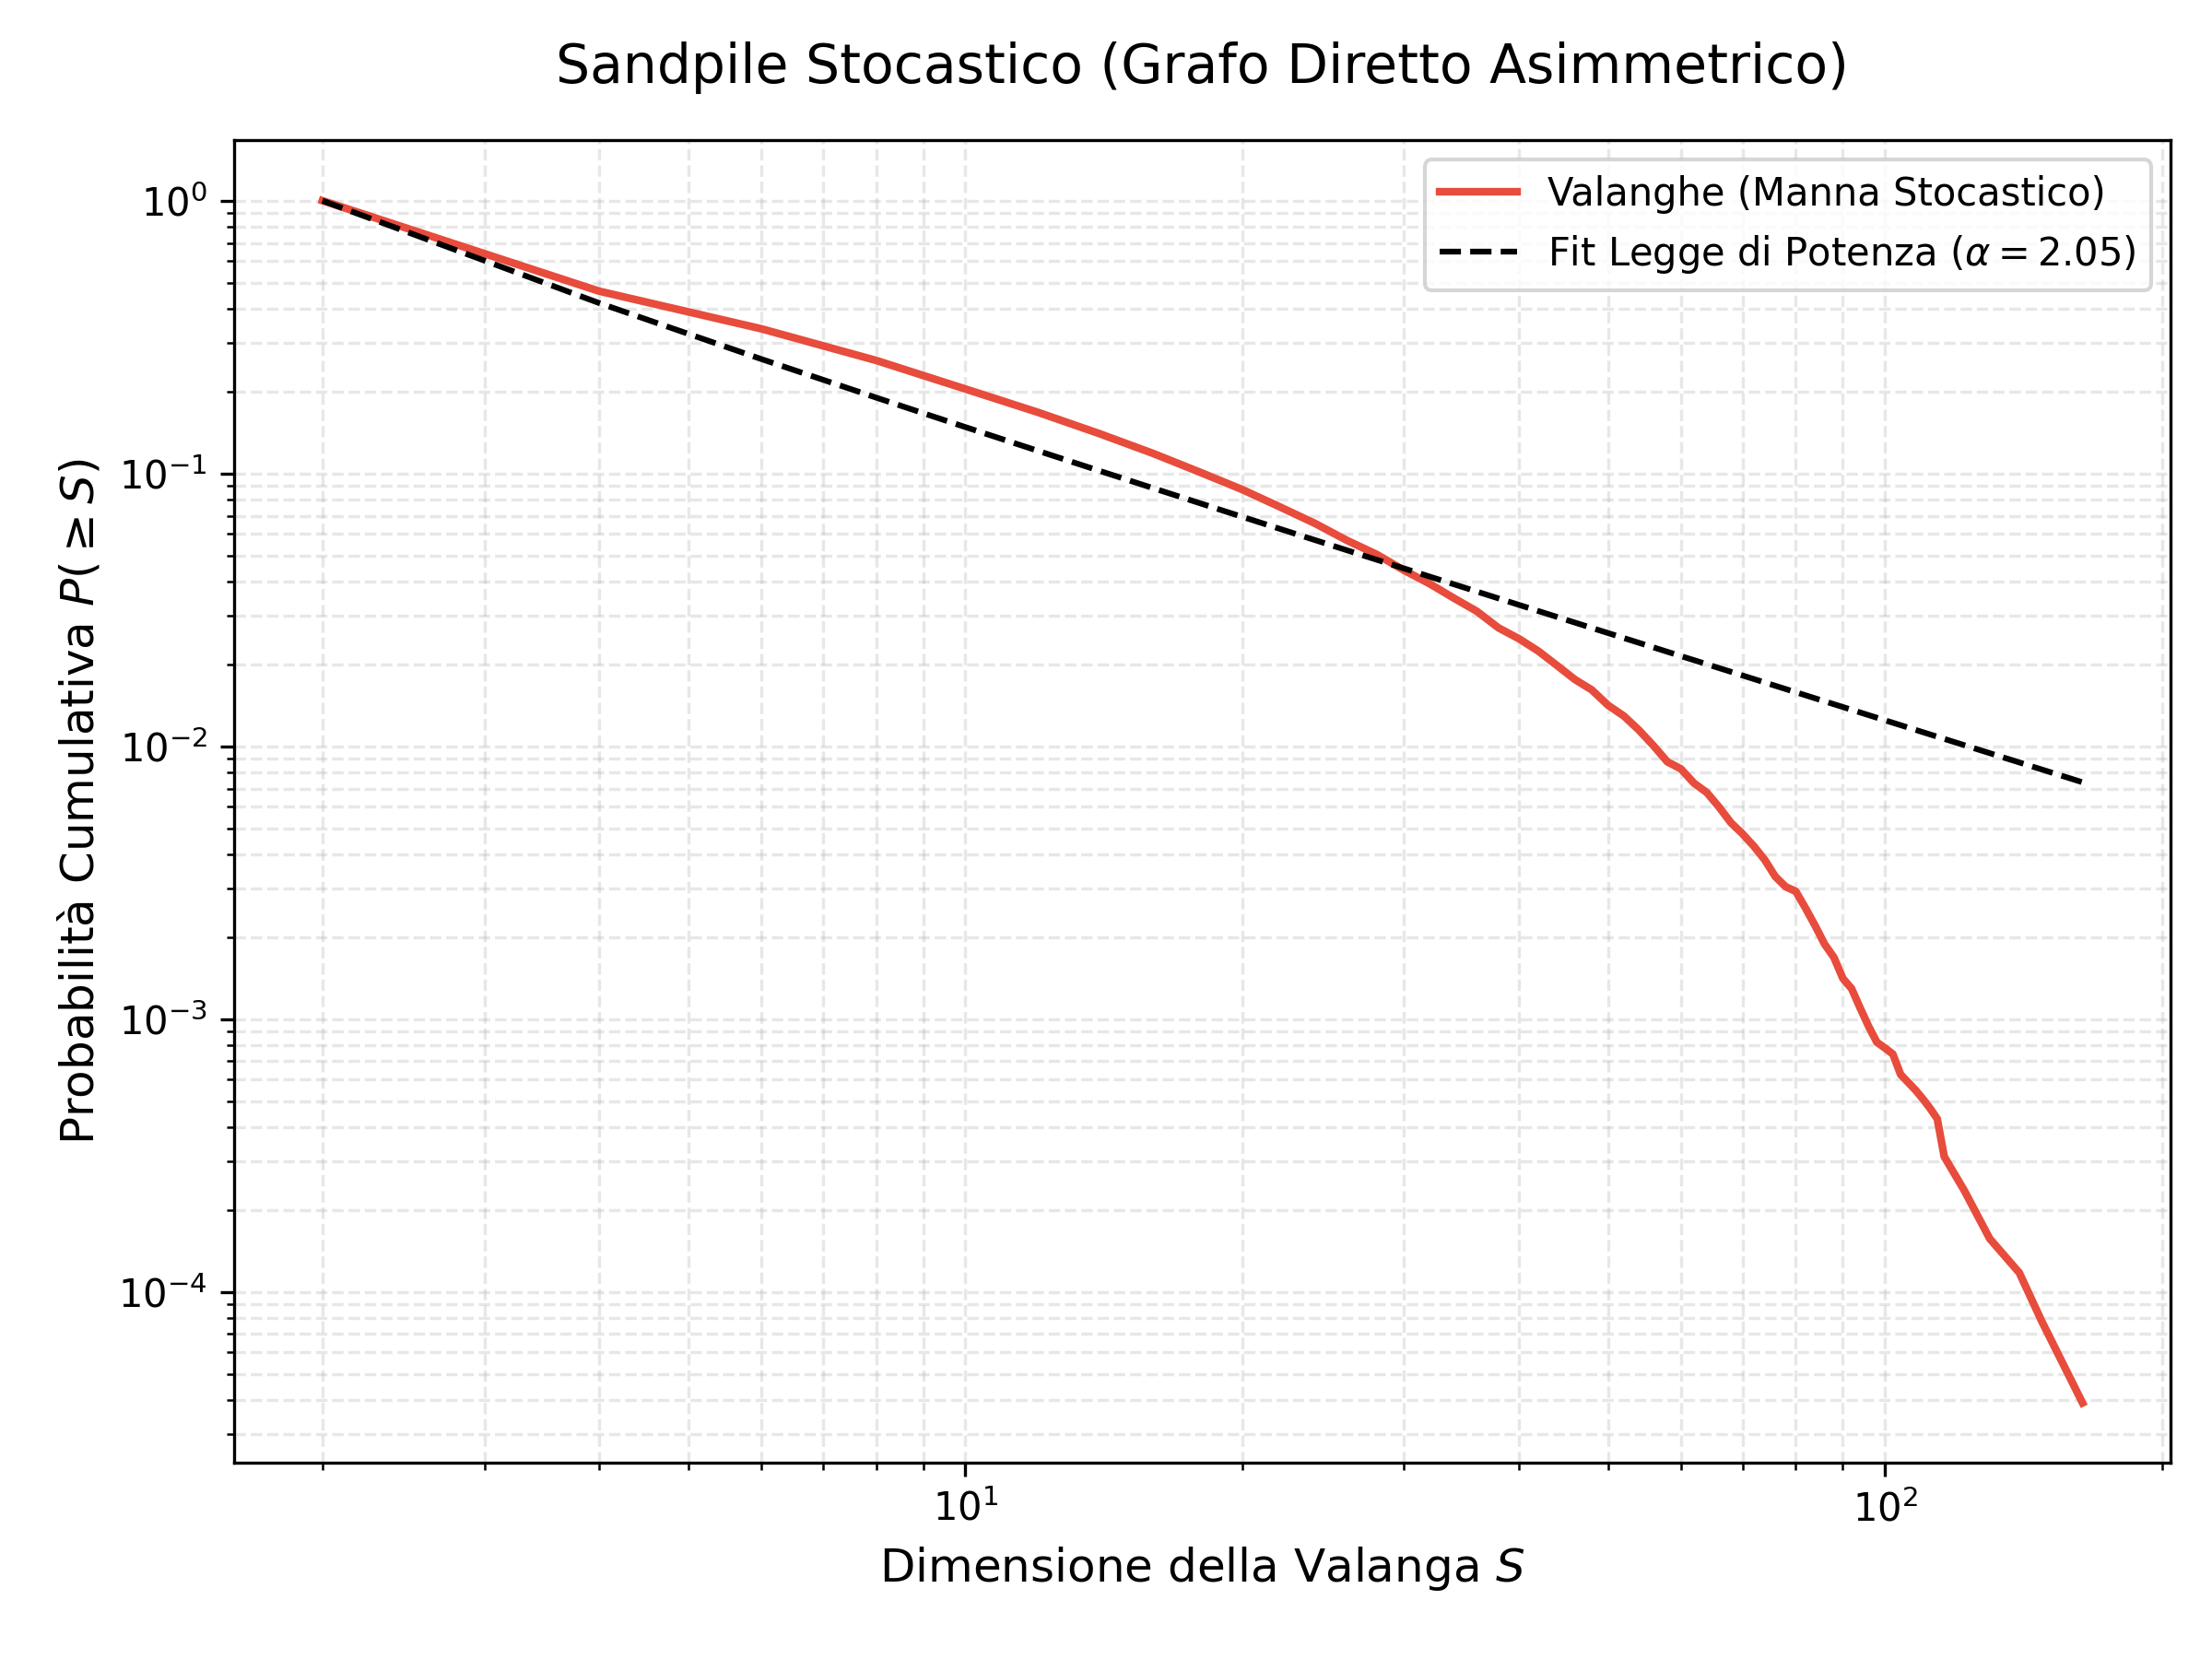
\includegraphics[width=0.85\textwidth]{manna_powerlaw.png}
\caption{Sandpile stocastico di Manna su grafo asimmetrico diretto. Eseguendo 5 replicazioni indipendenti sullo stesso sottografo ($N=1000$, estratto via BFS dalla componente connessa), le valanghe seguono stabilmente una legge di potenza ($\alpha = 2.065 \pm 0.005$). Il margine d'errore così piccolo riflette solo la stabilità su questa specifica topologia (5 run sullo stesso grafo), non una validità generale. In ogni caso il comportamento a legge di potenza resiste anche reintroducendo la direzionalità e i pesi reali delle associazioni, superando il limite del modello BTW simmetrico.}
\label{fig:manna}
\end{figure}

\newpage
\appendix
\section{Formule del modello}

Il sandpile vive su un grafo non orientato $G=(V,E)$; $\sigma(v)$ è il numero di grani sul nodo
$v$, $\deg(v)$ il suo grado, $\mathcal{N}(v)$ i suoi vicini.

\textbf{Regola di toppling.} Un nodo è instabile quando la quantità di grani accumulati supera la soglia. In tutti gli esperimenti e simulazioni riportate è stata utilizzata unicamente la convenzione stretta (parametro \texttt{strict=True}):
\[
\text{instabile se}\quad \sigma(v) > \deg(v)
\]
Quando crolla, il nodo cede un grano a ciascun vicino (conservativo):
\[
\sigma(v)\leftarrow \sigma(v)-\deg(v),\qquad
\sigma(u)\leftarrow \sigma(u)+1\quad \forall u\in\mathcal{N}(v).
\]
La regola è quella BTW \cite{bak1987} generalizzata a grafo arbitrario \cite{dhar1990}; è
\emph{abeliana}: la configurazione finale non dipende dall'ordine dei crolli.

\textbf{Dissipazione.} I grani lasciano il sistema in due modi: al \emph{sink} (un nodo designato che assorbe i grani in eccesso, equivalente al bordo aperto nel modello BTW) e/o tramite \emph{dissipazione di bulk}: ogni grano trasferito sparisce con probabilità $f$. Per l'analisi della criticità ho sempre mantenuto $f=0$ (modello deterministico).

\textbf{Massa massima stabile e regime caotico.} La massima quantità di grani che un nodo può ospitare senza crollare dipende dal suo grado. Di conseguenza, la massa totale che l'intera rete può contenere in modo stabile è:
\[
\texttt{max\_stable\_mass}=\sum_{v\neq\text{sink}}\big(\text{soglia}(v)-1\big).
\]
In un sistema chiuso (senza sink, $f=0$), non appena la somma dei grani supera questo limite matematico (che con la convenzione \texttt{strict=True} equivale esattamente alla somma dei gradi $\sum \deg(v)$), la configurazione non ammette più una stabilizzazione finita (regime supercritico). Questa formula è usata nel codice come base per intercettare ed evitare blocchi computazionali.

\textbf{Taglia della valanga.} $S=\sum_{v\ \text{crollati}}\deg(v)$ corrisponde al numero totale di grani spostati. Spesso in letteratura la taglia è il semplice numero di crolli, ma ho preferito usare i grani spostati per catturare l'effettivo volume di attivazione in gioco. Su reti così irregolari, questa scelta cambia il valore dell'esponente $\alpha$ che andiamo a misurare. In regime critico, la distribuzione segue $P(S\ge s)\propto s^{-(\alpha-1)}$.

\textbf{Transizione di fase.} Fissando la densità di grani $\rho=\sigma_{\text{tot}}/N$, si osserva l'attività stazionaria $\rho_a$ (la frazione di nodi in crollo). Sotto la soglia $\rho_c$, l'attività si spegne ($\rho_a=0$); sopra la soglia, persiste ($\rho_a>0$). Sul reticolo classico 2D la soglia è $\rho_c\approx 2.125$; se per caso le mie stime su rete semantica si avvicinano a questo numero, è un puro accidente numerico. Aggiungendo grani lentamente dall'esterno, il sistema si spinge spontaneamente verso questa densità critica \cite{dickman2000}.

\textbf{Dettagli Metodologici.} Le simulazioni sono state eseguite su sottografi estratti via BFS dalla rete SWOW gigante, con seme casuale fisso (\texttt{seed=42}) per la riproducibilità. Per il Finite-Size Scaling sono state raccolte tra le 1800 e le 3500 valanghe per rete (taglie $N \in \{250, 500, 1000, 2500\}$). I test sulla legge di potenza hanno utilizzato $N=1500$, con un burn-in iniziale pari alla somma dei gradi (alcune decine di migliaia di passi) per approssimare lo stato stazionario, raccogliendo poi $\sim 2900$ valanghe. La transizione di fase è stata calcolata su $N=1000$; l'effetto fan su $N=500$ con probe non distruttivo (background ripristinato dopo ogni nodo, per evitare contaminazioni). Gli errori e gli intervalli di confidenza sulla legge di potenza derivano dalla deviazione standard stimata dal pacchetto \texttt{powerlaw}.

\section{Codice: \texttt{sandpile.py}}

Implementazione (estratti dei metodi chiave). La soglia critica per nodo è precalcolata in
\texttt{crit}; un nodo è instabile se $\sigma(v)\ge\texttt{crit}[v]$.

\begin{lstlisting}
def __init__(self, graph, sink=None, f=0, strict=True, max_topplings=None):
    self.sink, self.f, self.strict = sink, f, strict
    self.non_sink_nodes = [n for n in graph.nodes if n != sink]
    self.node_degree = {n: graph.degree(n) for n in graph.nodes}
    # crit[v] = deg(v)+1 (strict=True, instabile se sigma > deg)
    #         = deg(v)   (strict=False, instabile se sigma >= deg, BTW classico)
    # in entrambi i casi il check e' sempre: sigma >= crit[v]
    self.crit = {n: self.node_degree[n] + (1 if strict else 0) for n in graph.nodes}
    # tetto oltre cui un sistema chiuso non puo' piu' stabilizzarsi
    self.max_stable_mass = sum(self.crit[n] - 1 for n in self.non_sink_nodes
                               if self.node_degree[n] > 0)
    self.max_topplings = max_topplings or 10 * len(self.non_sink_nodes)

def _unstable(self, status):
    # nodi che raggiungono la soglia di crollo
    return [v for v in self.non_sink_nodes
            if self.node_degree[v] > 0 and status[v] >= self.crit[v]]

def _topple(self, status):
    # crolli in round paralleli finche' il sistema e' stabile
    total_topplings, avalanche_size, toppled = 0, 0, set()
    unstable = self._unstable(status)
    while unstable:
        if total_topplings >= self.max_topplings:   # divergenza: stop
            return {"diverged": True, ...}
        for v in unstable:
            status[v] -= self.node_degree[v]         # cede deg(v) grani
            toppled.add(v); total_topplings += 1
            avalanche_size += self.node_degree[v]
            for u in self.node_neighbors[v]:
                if u == self.sink:        continue   # assorbito dal sink
                if self.f > 0 and np.random.random() < self.f: continue  # dissipato
                status[u] += 1                       # arriva al vicino
        unstable = self._unstable(status)
    return {"diverged": False, "avalanche_size": avalanche_size, ...}

def iteration(self, node=None):
    # un passo: aggiungi un grano su un nodo (casuale se None) e topple
    actual = dict(self.status)
    self._add_grain(actual, node)            # +1 su un nodo non-sink
    av = self._topple(actual)
    if av["diverged"]:
        return {..., "diverged": True}       # stato NON salvato, simulazione si ferma
    self.status = actual                     # commit
    return {..., "avalanche_size": av["avalanche_size"], "diverged": False}
\end{lstlisting}

\textbf{Pipeline degli esperimenti.} (1) Si costruisce $G$ da SWOW (componente connessa, sottografo
BFS per controllare la taglia). (2) \emph{Burn-in} di $K=\sum_v\deg(v)$ passi per raggiungere lo
stato stazionario \cite{dhar1990}. (3) Si misurano le taglie di valanga, l'attività $\rho_a$, la
densità $\rho(t)$. (4) Il fit a legge di potenza usa la libreria \texttt{powerlaw} (MLE con $x_{\min}$
scelto via Kolmogorov--Smirnov).

\begin{thebibliography}{6}
\bibitem{anderson1974} Anderson, J. R. (1974). Retrieval of propositional information from long-term memory. \emph{Cognitive psychology}, 5(4), 451-474.
\bibitem{bak1987} Bak, P., Tang, C., \& Wiesenfeld, K. (1987). Self-organized criticality: An explanation of the 1/f noise. \emph{Physical review letters}, 59(4), 381.
\bibitem{beggs2003} Beggs, J. M., \& Plenz, D. (2003). Neuronal avalanches in neocortical circuits. \emph{Journal of neuroscience}, 23(35), 11167-11177.
\bibitem{clauset2009} Clauset, A., Shalizi, C. R., \& Newman, M. E. (2009). Power-law distributions in empirical data. \emph{SIAM review}, 51(4), 661-703.
\bibitem{dedeyne2019} De Deyne, S., Navarro, D. J., Perfors, A., Brysbaert, M., \& Storms, G. (2019). The ``Small World of Words'' English word association norms for over 12,000 cue words. \emph{Behavior research methods}, 51(3), 987-1006.
\bibitem{dhar1990} Dhar, D. (1990). Self-organized critical state of sandpile automaton models. \emph{Physical review letters}, 64(14), 1613.
\bibitem{dickman2000} Dickman, R., Muñoz, M. A., Vespignani, A., \& Zapperi, S. (2000). Paths to self-organized criticality. \emph{Brazilian Journal of Physics}, 30(1), 27-41.
\end{thebibliography}

\end{document}
